
\part{The Jacobian Problem}\label{part2}

\chapter{The Jacobian Problem}\label{part2:chap6}

\setcounter{section}{14}
\section{Statement of the Problem}\label{part2:chap6:sec15}

\subsection{}\label{part2:chap6:sec15:ss15.1}

\setcounter{pageoriginal}{116}

Let\pageoriginale $k$ be a field and let $A= k[x_1, x_2]$ be the
polynomial ring in two variables $x_1$, $x_2$ over $k$. Let $K$ be the
quotient field of $A$. $A$ pair $(u_1, u_2)$ of elements of $A$ is an
{\em automorphic pair} (for $A$) if $A= k[u_1, u_2]$. Note that $(u_1,
u_2)$ is an automorphic pair if and only if the $k$-algebra
homomorphism $\sigma : A \to A$ defined by $\sigma (x_i) = u_i$, $i=1,
2$, is an automorphism. $A$ pair $(u_1, u_2)$ of elements of $K$ is a
{\em transcendence base} (of $K$ over $k$) if $K$ is algebraic over
$k(u_i , u_2)$. Clearly, every automorphic pair is a transcendence
base.

Let $u= (u_1, u_2)$ be a transcendence base. Then $u_1, u_2$ are
algebraically independent over $k$. Therefore there exist
$k$-derivations $D_{u, 1}$, $D_{u, 2}$ of $k(u_1, u_2)$ defined by
$D_{u, i}(u_j)= \delta_{ij}$ (Kronecker delta). Suppose now that $K$
is separable over $k(u_1, u_2)$. Then for each $i= 1, 2, D_{u, i}$
extends to a unique $k$-derivation of $K$. We shall denote this
extension also by $D_{u, i}, i=1, 2$. In particular, for each
automorphic pair $u= (u_1, u_2)$ we have $k$-derivations $D_{u,i}$ of
$K$, $i=1, 2$. We shall often write simply $D_i$ for $D_{x,i}$, $i=1,
2$, where $x= (x_1, x_2)$. Note that if $u$ is an automorphic pair
then $d_{u, i}(A) \subset A$, $i=1,2$. 

\setcounter{thm}{1}
\begin{defi}\label{part2:chap6:sec15:def15.2}
  Let $u= (u_1, u_2)$ be an automorphic pair and let $f$, $g \in
  A$. The {\em Jacobian of $(f, g)$ with respect to} $u$, denoted
  $J_u(f, g)$, is defined by
  $$
  J_u (f, g)= \det 
  \begin{pmatrix} 
    D_{u, 1} (f) & D_{u, 2}(f)\\
    D_{u, 1}(g) & D_{u, 2}(g)
  \end{pmatrix}
  = D_{u, 1} (f) D_{u, 2}(g) - D_{u, 2}(f) D_{u,1}(g).
  $$
  We shall write simply $J(f, g)$ for $J_x (f, g)$. 
\end{defi}

\begin{lemma}\label{part2:chap6:sec15:lem15.3}
  Let\pageoriginale $u= (u_1, u_2)$, $v= (v_1, v_2)$ be automorphic pairs for $A$
  and let $f$, $g \in A$. Then we have
  $$
  J_{u}(f, g)= J_v (f, g) J_u (v_1, v_2). 
  $$
\end{lemma}

\begin{proof}
  This is immediate from the chain rule for derivations, namely 
  $$
  D_{u,i}(a)=D_{u, 1} (a) D_{u, i} (v_1)+ D_{v, 2}(a) D_{u, i} (v_2) ~
  \text{ for }~ a \in A, i=1,2.
  $$
\end{proof}

\begin{coro}\label{part2:chap6:sec15:coro15.4}
  Let $u= (u_1, u_2)$, $v= (v_1, v_2)$ be automorphic pairs for
  $A$. Then $J_u (v_1, v_2)$ is a unit of $A$.
\end{coro}

\begin{proof}
  By Lemma \ref{part2:chap6:sec15:lem15.3} we have
  $$
  1= J_u (u_1, u_2)= J_{v}(u_1, u_2) J_u (v_1, v_2)
  $$
  and the corollary is proved.
\end{proof}

\setcounter{subsection}{4}
\subsection{}\label{part2:chap6:sec15:ss15.5}

Noting that the units of $A$ are the non-zero elements of $k$, it
follows from Corollary \ref{part2:chap6:sec15:coro15.4} that if $(f,
g)$ is an automorphic pair for $A$ then $J(f, g)$ is a non-zero
element of $k$. Then Jacobian problem asks whether the converse is
true in case char $k=0$:

\noindent \textbf{The Jacobian Problem.} Suppose char $k=0$. Let $f,
g$ be elements of $A$ such that $J(f, g)$ is a non-zero element of
$k$. Is $(f, g)$ then an automorphic pair for $A$?

\setcounter{thm}{5}
\begin{remark}\label{part2:chap6:sec15:rem15.6}
  Suppose char $k=p > 0$. Let $f = x_1 + x_1^p$, $g= x_2$. Then $J(f,
  g)=1$. Then $J(f, g)=1$. However, $(f, g)$ is not an
  automorphic pair. For, $k[x_1, x_2]/(g)=k[x_1]\neq k[x_1 + x_1^p]$,
  which shows that $k[f, g]\neq k[x_1, x_2]$. This explains the
  assumption char $k=0$ made in the Jacobian problem.
\end{remark}

\section{Notation}\label{part2:chap6:sec16}

\subsection{}\label{part2:chap6:sec16:ss16.1} 

Let\pageoriginale $A= k[x_1, x_2]$ as in
\S\ \ref{part2:chap6:sec15}. {\em We assume henceforth that} char
$k=0$. Let $w= (w_1, w_2)$ be a pair of integers. By the $w$-{\em
  gradation} on $A$ we mean the gradation on $A$ obtained by giving
weight $w_i$ to $x_i$, $i=1,2$. Recall that this means that we write
$A$ in the form
$$
A= \mathop{\oplus}_{n \in \mathbb{Z}} A_w^{(n)},
$$
where $A_w^{(n)}$ is the $k$-subspace of $A$ generated by monomials
$x_1^{i_1} x_2^{i_2}$ with $i_1 w_1 + i_2 w_2=n$. The elements of
$A_w^{(n)}$ are called $w$-{\em homogeneous} elements of $w$-{\em
  degree} $n$. Note that by this definition 0 is $w$-homogeneous of
$w$-degree $n$ for every $n$. Every element $f$ of $A$ can be written
uniquely in the form $\displaystyle{f= \sum_n f_w^{(n)}}$, where
$f_n^{(n)}$ is $w$-homogeneous of $w$-degree $n$ and $f_w^{(n)}=0$
for almost all $n$. We call $f_w^{(n)}$ the $n^{\rm th}$ $w$-{\em homogeneous
  component} of $f$. Suppose $f \neq 0$. Then there exists $m\in
\mathbb{Z}$ such that $f_w^{(m)} \neq 0$ and $f_w^{(n)}=0$ for all $n
> m$. We call this $m$ the $w$-{\em degree} of $f$ and denote it by
$d_w (f)$. Thus
$$
d_w (f) = \sup \left\{ n \in \mathbb{Z} \big| f_w^{(n)} \neq 0 \right\}.
$$

If $f=0$, we define $d_w (f)= - \infty$. If $f \neq 0$ then the
$w$-{\em degree form} of $f$, denoted $f_w^+$, is defined by $f_w^+=
f_w ^{(m)}$, where $m=d_w (f)$. If $f=0$, we define $f_w^+=0$. Note
that $f$ is $w$-homogeneous if and only if $f= f_w^+$. 

Suppose now that $w= (1, 1)$. then the $w$-gradation on $A$ is called
the {\em usual gradation} on $A$. In this case we often omit the
symbol $w$ in the notation introduced above. Thus we write $d(f)$,
$f^{(n)}$, $f^+, \ldots $ etc. for $d_w(f), f_w^{(n)}$, $f_w^+,
\ldots$. when $w= (1, 1)$.

\subsection{}\label{part2:chap6:sec16:ss16.2}

The\pageoriginale $w$-gradation on $A$ defined in
\ref{part2:chap6:sec16:ss16.1} above is with respect to the
automorphic pair $x= (x_1, x_2)$. If $u= (u_1, u_2)$ is any
automorphic pair then we can also define a gradation on $A$ by giving
weight $w_i$ to $u_i$, $i=1, 2$. However, in the sequel we will mostly
need to consider only the $(1,1)$-gradation on $A$ with respect to an
arbitrary automorphic pair $u$. In order to distinguish this from the
usual gradation, we fix the following notation:

\begin{tabbing}
  \qquad\qquad  \= $\deg f $ \; \= {\em denotes} $d_{(1,1)}(f)$ with
  respect to $x$,\\ 
   \> $\deg_u f $~ \> {\em denotes }~ $d_{(1,1)}(f)$ with respect to $u$,
\end{tabbing}

If $u=(u_1, u_2)$ is an automorphic pair and $f \in A$, we write
$\deg_{u_1} f$ (\resp $\deg_{u_2}f$) for the $u_1$- degree (\resp
$u_2$-degree) of $f$ regarded as a polynomial in $u_1$ (\resp $u_2$)
with coefficients in $k[u_2]$ (\resp $k[u_1]$).

\subsection{} \label{part2:chap6:sec16:ss16.3}

One final piece of notation: We denote by $k^*$ the set of non-zero
elements of $k$ and, as noted in \ref{part1:chap3:sec7:notn7.2}, we
use the symbol $\diameter$ to denote a generic (i.e., unspecified
element of $k^*$.)

\section{$w$-Relation}\label{part2:chap6:sec17}

We preserve the notation of \S \ref{part2:chap6:sec15} and
\S \ref{part2:chap6:sec16}. In particular, we have char $k=0$. Let $w=
(w_1, w_2)$ be a pair of integers. 

\begin{lemma}\label{part2:chap6:sec17:lem17.1}
  Let $F$, $G$ be non-zero $w$-homogeneous elements of $A$. The
  following two conditions are equivalent:
  \begin{enumerate}[\rm (1)]
    \item $F^r = \diameter G^s$ for some $r, s \in \mathbb{Z}^+$;
      $r+s> 0$.
      \item There exist $p$, $q \in \mathbb{Z}^+$ and a
        $w$-homogeneous element $H$ of $A$ such that $F= \diameter
        H^p$, $G= \diameter H^q$.
  \end{enumerate}
\end{lemma}

\begin{proof}
  (1)\pageoriginale $\Rightarrow$ (2). Write $F= \diameter H_1^{p_1}\ldots
  H_n^{p_n}$, $G= \diameter H_1^{q_1}\ldots H_n^{q_n}$, where $H_i$ is
  an irreducible $w$-homogeneous element of $A$, $p_i$, $q_i \in
  \mathbb{Z}^+$ for $1 \leq i \leq n$ and \gcd $(H_i, H_j)= 1$ for $i
  \neq j$. Then (1) implies that $rp_i= sq_i$ for every $i$, $1 \leq i
  \leq n$. Now, if $r=0$ or $s=0$, say $r=0$, then $s> 0$ and $q_i =0$
  for every $i$, so that $G = \diameter$. In this case (2) follows by
  taking $H= F$, $p=1$, $q=0$. We may therefore assume that $r> 0$ and
  $s> 0$. Then for any $i$, $p_i=0$ if and only if $q_i =0$. Therefore
  we may assume that $p_i > 0$ and $q_i > 0$ for every $i$, $1 \leq i
  \leq n$. Then for every $i$ we have $p_i/ q_i= s/r= p/q$, say, where
  $p, q$ are positive integers such that \gcd $(p, q)=1$. For every
  $i$, $1 \leq i \leq n$, there exists a positive integer $t_i$ such
  that $p_i= p t_i$, $q_i = qt_i$. Let $H= H_1^{t_1} \ldots
  H_n^{t_n}$. Then $F= \diameter H^p$, $G= \diameter H^q$. 

(2) $\Rightarrow$ (1). If $p=0=q$ then $F = \diameter$, $G=
  \diameter$, so that $F= \diameter G$, which implies (1) in this
  case. Assume therefore that $p+q> 0$. Now, (2) implies that $F_q =
  \diameter G^p$, which implies (1).
\end{proof}

\begin{defi}\label{part2:chap6:sec17:def17.2}
  Let $f$, $g \in A$. We say $f$ and $g$ are $w$-{\em related} if $f
  \neq 0$, $g\neq 0$, and $F = f_w^+$ and $g= g_W^+$ satisfy the
  equivalent conditions (1) and (2) of  Lemma
  \ref{part2:chap6:sec17:lem17.1}. We say $f$ and $g$ are {\em
    related} if $f$ and $g$ are (1,1)-related. 
\end{defi}

\begin{lemma}\label{part2:chap6:sec17:lem17.3}
  Let $f, g_1 , \ldots, g_e$ be elements of $A$.
  \begin{enumerate}[\rm (i)]
    \item If $f_w^+= \diameter$ and $g_1 \neq 0$ then $f$ and $g_1$
      are $w$-related.
      \item If $f$ and $g_i$ are $w$-related for every $i$, $1 \leq i
        \leq e$, then $f$ and $g_1 \ldots g_e$ are $w$-related.
  \end{enumerate}
\end{lemma}

\begin{proof}
  ~
\begin{enumerate}[(i)]
  \item We have $f_w^+= \diameter = \diameter (g_{1w}^+)^\circ$.
    \item By induction on $e$, it is enough to consider the case
      $e=2$. There exist $r_i$, $s_i \in \mathbb{Z}^+$, $r_i + s_i >
      0$, such that $F^{r_i}= \diameter G_i^{s_i}$, where $F= f_w^+$,
      $G_i = g_{iw}^+$, $i= 1, 2$. This gives
      \begin{equation*}
        F^{r_1 s_2 + r_2 s_1} = \diameter (G_1 G_2)^{s_1
          s_2}. \tag{17.3.1} \label{part2:chap6:sec17:eq17.3.1}
      \end{equation*}
\end{enumerate}

If\pageoriginale $s_i=0$ for $i=1$ or 2, say $s_1=0$, then $r_1 > 0$
and $F^{r_1}= \diameter G_1^\circ= \diameter$ shows that $F=
\diameter$. Therefore in this case $f$ is related to $g_1 g_2$ by
(i). We may therefore assume that $s_1> 0$, $s_2> 0$. Then $s_1 s_2 >
0$, and it follows from (\ref{part2:chap6:sec17:eq17.3.1}) that $f$
and $g_1 g_2$ are $w$-related.
\end{proof}

\begin{prop}\label{part2:chap6:sec17:prop17.4}
  Let $F$, $G$ be non-zero $w$ - homogeneous elements of $A$ of
  $w$-degrees $m$, $n$, respectively. Consider the following five
  conditions:
  \begin{enumerate}
  \renewcommand{\labelenumi}{(\theenumi)}
  \item $F$ and $G$ are $w$-related.
    \item $F$ and $G$ are algebraically dependent over $k$.
      \item $J(F, G)=0$.
        \item $F^n = \diameter G^m$.
          \item $F^{|n|}= \diameter G^{|m|}$.

  Among these five conditions we have the following implications:

(1) $\Rightarrow$ (2) $\Rightarrow$ (3) $\Rightarrow$ (4)
  $\Rightarrow$ (5).

Assume, moreover, that at least one of the following two conditions is
satisfied:

(i) $w_1 w_2 > 0$ and $F \notin k$ or $G \notin k$.

(ii) $m \neq 0$ or $n \neq 0$.

Then the above five conditions (1) - (5) are equivalent to each
other. Further, let $d=\text{\gcd}~ (m, n)$. Then $d > 0$ and the
conditions (1) - (5) are also equivalent to each of the following two
conditions: 
\item $F^{n/d}= \diameter G^{m/d}$.
  \item We have $mn \geq 0$ and there exists a $w$-homogeneous element
    $H$ of $A$ such that $F= \diameter H^{|m|/d}, G= \diameter H^{|n|/d}$.
  \end{enumerate}
\end{prop}

In\pageoriginale order to prove the proposition, we need the following
three lemmas:

\setcounter{mysubsection}{14}
\subsubsection{\textbf{LEMMA.}} \label{part2:chap6:sec17:sss17.4.1}

Let $L$ be a field and let $L(t)$ be
the field of rational functions in one variable $t$ over $L$. Let
$D_t$ be the $L$-derivation of $L(t)$ defined by $D_t(t)=1$. If $h$ is
an element of $L(t)$ such that $D_t(h)=0$ then $h \in L$.

\subsubsection{\textbf{LEMMA.}} \label{part2:chap6:sec17:sss17.4.2}

Let $f$, $g$ be non-zero elements of $A$ of $w$-degrees $m$, $n$,
respectively. If $f^n = \diameter g^m$ then $mn \geq 0$. 

\subsubsection{\textbf{LEMMA.}} \label{part2:chap6:sec17:sss17.4.3}

Let $F$, $G$ be non-zero $w$ homogeneous elements of $A$ of
$w$-degrees $m$, $n$ respectively. Then we have:
\begin{enumerate}[(i)]
\item ~
\vskip -1.5cm
\begin{align*}
  mF & = w_1 x_1 D_1 (F) + w_2 x_2 D_2 (F),\\
  nG & = w_1 x_1 D_1 (G) + w_2 x_2 D_2 (G).
\end{align*}
\item ~
\vskip -1.5cm
\begin{align*}
  w_1 x_1 J(F, G) & = m F D_2 (G) - nG D_2 (F),\\
  w_2 x_2 J(F, G) & = nG D_1 (F) - mF d_1 (G).
\end{align*}
\end{enumerate}

\medskip
\noindent\textbf{Proof of Lemma \ref{part2:chap6:sec17:sss17.4.1}.}
The assertion is clear if $h \in L [t]$. In general, we can write $h=
f/g$ with $f$, $g \in L [t]$ and \gcd $(f, g)=1$. Then we have
$$
0 = D_t (h) = (g D_t (f) - fD_t (g))/g^2,
$$ 
which shows that $g D_t (f) = fD_t (g)$. Thus $g$ divides $fD_t (g)$
in $L[t]$. Therefore, since \gcd $(f, g)=1$, $g$ divides $D_t
(g)$. Since $\deg_t D_t (g) < \deg_t g$, we get $D_t (g) =0$, so that
$g \in L$. Therefore $h \in L [t]$, and the assertion follows.

\medskip
\noindent \textbf{Proof of Lemma \ref{part2:chap6:sec17:sss17.4.2}.}
Suppose $mn< 0$. then one of $m$, $n$ is positive and the other is
negative. We may suppose that $m < 0$ and $n> 0$. Then $f^n g^{-m}=
\diameter$ implies that $f$ (also $g$) is a unit of $A$. Therefore $f
\in k^*$. But this means that $m =0$,\pageoriginale which is a
contradiction.

\medskip
\noindent \textbf{Proof of Lemma \ref{part2:chap6:sec17:sss17.4.3}.} 
(i) We have only to observe that
$$
w_1 x_1 D_1 \left( x_1^{i_1} x_2^{i_2}\right)+ \omega_2 x_2 D_2
\left(x_1^{i_1} x_2^{i_2} \right) = \left(i_1 w_1 + i_2 w_2 \right)
x_1^{i_1}  x_2^{i_2}.
$$

(ii) We have
\begin{align*}
  w_1 x_1 J(F, G) & = \det 
  \begin{pmatrix}
    w_1 x_1 D_1 (F) & D_2 (F)\\
    w_1 x_1 D_1 (G) & D_2 (G)
  \end{pmatrix}\\
  & = \det 
  \begin{pmatrix}
    w_1 x_1 D_1 (F)+ w_2 x_2 D_2 (F) & D_2 (F)\\
    w_1 x_1 D_1 (G) + w_2 x_2 D_2 (G) & D_2 (G)
  \end{pmatrix}\\
  & = \det 
  \begin{pmatrix}
    mF & D_2 (F)\\
    nG & D_2 (G)
  \end{pmatrix} \qquad (\text{by (i)})\\
  & = m ~ F D_2 (G) - n G D_2 (F).
\end{align*}
This proves the first equality of (ii). The second is proved
similarly.

\medskip
\noindent \textbf{Proof of Proposition \ref{part2:chap6:sec17:prop17.4}.} 
(1) $\Rightarrow$ (2). We have
$F^r = \diameter G^s$ for some non-negative  integers $r$, $s$, $r+s>
0$. Therefore $F$ and $G$ are algebraically dependent over $k$.

(2) $\Rightarrow$ (3). Let $X_1$, $X_2$ be indeterminates and let
$\varphi= \varphi (X_1, X_2)\in k[X_1, X_2]$ be such that $\varphi
\neq 0$ and $\varphi (F, G)=0$. Then $\varphi \notin k$. Therefore
$\deg_{X_1} \varphi+ \deg_{X_2}\varphi > 0$. We may choose $\varphi$
to be such that $\deg_{X_1} \varphi+ \deg_{X_2}\varphi$ is the least
possible. Let $\varphi_i = D_{X, i}(\varphi)$, $i=1, 2$, where $X=
(X_1, X_2)$. Then we have $\deg_{X_1} \varphi_i + \deg_{X_2}
\varphi_1< \deg_{X_2}\varphi+ \deg_{X_2}\varphi$, $i= 1, 2$. Moreover
$\varphi_1 \neq 0$ or $\varphi_2\neq 0$.\pageoriginale Ir follows that
we have $\varphi_1 (F, G)\neq 0$ or $\varphi_2 (F, G) \neq 0$. Now, we
have
\begin{align*}
  0 & = D_1 (\varphi (G, G)) = \varphi_1 (F, G) D_1 (F)+ \varphi_2 (F,
  G)D_1 (G),\\
  0 & = D_2 (\varphi (F, G)) = \varphi_1 (F, G)D_2 (F) + \varphi_2 (F,
  G) D_2 (G).
\end{align*}

Since $\varphi_1 (F, G) \neq 0$ or $\varphi_2 (F, G)\neq 0$, we get
$$
0 =\det 
\begin{pmatrix}
D_1 (F) & D_1 (G)\\
D_2 (F) & D_2 (G)
\end{pmatrix} = J(F, G),
$$
which proves (3).

(3) $\Rightarrow$ (4). We have $J(F, G)=0$ and we want to show that
$F^n/G^m \in k$. Since $k= k(x_1) \cap k(x_2)$, it is enough, by
symmetry, to show that $F^n/G^m \in k(x_1)$. By
lemma \ref{part2:chap6:sec17:sss17.4.3}, we have
$$
0 = w_1 x_1 J(F, G) = m F D_2 (G) - n G D_2 (F).
$$  

This gives 
$$
D_2 (F^n / G^m) = F^{n-1} G^{m-1} (n G D_2 (F)- m F D_2 (G))/G^{2m}=0.
$$

Therefore $F^n/ G^m \in k(x_1)$ by Lemma
\ref{part2:chap6:sec17:sss17.4.1}. 

(4) $\Rightarrow$ (5). Since $F^n = \diameter G^m$ if and only if
$F^{-n}= \diameter G^{-m}$, it is enough to show that we have $m \geq
0$, $n \geq 0$ or $m \leq 0$, $n \leq 0$. But this is immediate, since
$mn \geq 0$ by Lemma \ref{part2:chap6:sec17:sss17.4.2}.

Assume now that one of the conditions (i) and (ii) is satisfied. It is
then enough to prove that $d < 0$, (5) $\Rightarrow$ (1) and (1)
$\Rightarrow$ (7) $\Rightarrow$ (6) $\Rightarrow$ (2).

We first note that if condition (i) is satisfied then either $w_1 >
0$, $w_2 > 0$ or $w_1 < 0$, $w_2 < 0$. In either case, since $F \notin
k$ or $G \notin k$, we get $m \neq 0$ or $n \neq 0$. Therefore we may
assume that condition (ii) is satisfied. It is then clear
that\pageoriginale $d> 0$.

(5) $\Rightarrow$ (1). Trivial, since $m \neq 0$ or $n \neq 0$.

(1) $\Rightarrow$ (7). There exist $p$, $q \in \mathbb{Z}^+$ and a
$w$-homogeneous element $E$ of $A$ such that $F= \diameter E^p$, $G =
\diameter E^q$. Let $e = d_w (E)$. Then $m = pe$, $n = qe$. It
follows that $mn\geq 0$. Also, since condition (ii) is satisfied, we
have $p > 0$ or $q> 0$, say $q>0$. Let $d' =$\gcd $(p, q)$ and write
$p = p' d'$, $q= q'd'$, so that \gcd $(p' , q')=1$. Let $H=
E^{d'}$. Then $F= \diameter H^{p'}$, $G= \diameter H^{q'}$. It is now
enough to show that $p' = |m|/d$, $q'= |n|/d$. Since $q>0$ and since
$$
\text{\gcd} ~ (p', q')=1 = \text{\gcd}~ (|m|/d, |n|/d),
$$
it is enough to prove that $p' |n|= q'|m|$. Now, since $F= \diameter
E^p$, $G= \diameter E^q$, we have $pn = d_w (G^p) = d_w(E^{pq})=d_w
(F^q)= qm$. This shows that $p' |n|= q' |m|$.

(7) $\Rightarrow$ (6). Immediate, since $mn \geq 0$.

(6) $\Rightarrow$ (2). Immediate, since $m \neq 0$ or $n \neq 0$.

\begin{coro}\label{part2:chap6:sec17:coro17.5}
  Let $f$, $g_1, \ldots, g_e$ be non-zero elements of $A$. Let $m= d_w
  (f)$, $n_i =d_w (g_i)$, $1 \leq i \leq e$, and let $d=$ \gcd $(m,
  n_1 , \ldots , n_e)$. Assume that $m>0$ and that $f$ and $g_i$ are
  $w$ related for every $i$, $1 \leq i \leq e$. Then there exists a
  $w$-homogeneous element $H \in A$ of $w$-degree $d$ such that
  $f^+_w= \diameter H^{m/d}$.
\end{coro}

\begin{proof}
  We prove the assertion by induction on $e$. Since $f$ and $g_1$ are
  $w$-related, there exists, by Proposition
  \ref{part2:chap6:sec17:prop17.4}, a $w$-homogeneous element $H_1$ of
  $A$ such that $f_w^+ = \diameter H_1^{m/d_1}$, where $d_1 =$ \gcd
  $(m, n_1)$. It follows that $d_w (H_1)= d_1$, so that the assertion
  is proved for $e=1$. Now, let $e>1$ and let $d'=$ \gcd $(m, n_1,
  \ldots , n_{e-1})$, $d''$= \gcd $(m, n_e)$. By induction hypothesis
  and by the case $e=1$, there exist $w$-homogeneous elements $H_2$,
  $H_3$ of $A$ with $d_w (H_2)= d'$, $d_w (H_3)= d''$,\pageoriginale such that
  $f_w^+= \diameter H_2^{m/d'}= \diameter H_3^{m/d''}$. This shows
  that $H_2$ and $H_3$ are $w$-related. Therefore by the case $e=1$, there
  exists a $w$-homogeneous element $H \in A$ of $w$-degree $d$ such
  that $H_2= \diameter H^{d'/d}$. (Note that $d=$ \gcd $(d', d'')$.)
  Thus we get $f_w^+= H^{m/d}$.
\end{proof}

\section{Structure of the $w$-Degree Form}\label{part2:chap6:sec18}

We preserve the notation \S \ref{part2:chap6:sec15} and
\S \ref{part2:chap6:sec16}. In particular, we have char $k=0$. Let $w=
(w_1, w_2)$ be a pair of integers. 

\begin{defi}\label{part2:chap6:sec18:def18.1}
  For non-zero elements $f$, $g$ of $A$ we define
  $$
  \delta_w (f, g) = d_w (fg) - d_w (x_1 x_2)-d_w (J (f, g)).
  $$
\end{defi}

\begin{lemma}\label{part2:chap6:sec18:lem18.2}
  Let $f$, $g$ be non-zero elements of $A$. Then we have:
  \begin{enumerate}[(i)]
    \item $\delta_w (f, g)\geq 0$.
      \item $J(f_w^+, g_w^+) = \begin{cases} 
        J(f, g)_w^+, & \text{if}~ \delta_w (f, g) =0\\
        0, & \text{if}~ \delta_w (f, g)> 0.
      \end{cases}$
  \end{enumerate}
\end{lemma}

\begin{proof}
  ~
  \begin{enumerate}[(i)]
    \item Clearly, we have
      \begin{align*}
        d_w (D_i (f)) & \leq d_w (f) - w_i,\\
        d_w (D_i(g)) & \leq d_w (g) -w_i
      \end{align*}
      for $i=1, 2$. Therefore
      {\fontsize{10}{12}\selectfont
      $$
      d_w (D_1 (f) D_2 (g) - D_2 (f) D_1 (g)) \leq d_w (fg) - w_1 -
      w_2 = d_w (fg) -d_w (x_1 x_2).
      $$}
      which proves (i).

      \item Let\pageoriginale $f' = f- f^+_w$, $g'= g-g_w^+$. Then $d_w (f')< d_w
        (f)$, $d_w (g')< d_w (g)$. An easy computation shows that
        $$
        J(f, g)= J(f^+_w, g^+_w) +h.
        $$
        where $h \in A$ with $d_w (h) < d_w (fg)- d_w (x_1 x_2)$. Now,
        (ii) follows, since $J(f^+_w, g_w^+)$ is (either zero or)
        $w$-homogeneous of $w$-degree $d_w (fg)-d_w (x_1x_2)$.
  \end{enumerate}
\end{proof}

\begin{lemma}\label{part2:chap6:sec18:lem18.3}
  Let $f$ be a non-zero element of $A$ such that $d_w (f) \neq
  0$. Suppose there exists $g \in A$ such that $f$ and $J(f, g)$ are
  $w$-related. Then there exists $h \in A$ such that $f$ and $J(f, h)$
  are $w$-related and $\delta_w (f, h)=0$.
\end{lemma}

\begin{proof}
  If $\delta_w (f, g)=0$ then we may take $h=g$. Assume therefore that
  $\delta_w (f, g)> 0$. It is then enough to prove the following
  assertion:

\setcounter{subsubsection}{0}
\setcounter{mysubsection}{3}
\subsubsection{} \label{part2:chap6:sec18:sss18.3.1}
{\em There exists $h \in A$ such that $f$ and $J(f,
  h)$ are $w$-related and} $\delta_w (f, h)< \delta_w (f, g)$.

For, then the lemma would follow by induction on $\delta_w (f, g)$. To
prove \ref{part2:chap6:sec18:sss18.3.1}, we note first that, since $f$
and $J(f, g)$ are $w$-related, we have $j(f, g)$ are $w$-related, we
have $J(f, g)\neq 0$ by definition. Therefore $g \neq 0$. Moreover, by
Lemma \ref{part2:chap6:sec18:lem18.2} the assumption $\delta_w (f, g)>
0$ implies that $J(f_w^+, g_w^+)=0$. Therefore by Proposition
\ref{part2:chap6:sec17:prop17.4} $f$ and $g$ are $w$-related and there
exists $c \in k^*$ such that $c(f_w^+)^{|n|}= (g_w^+)^{|m|}$, where
$m= d_w (f)$, $n= d_w (g)$. (Note that by assumption we have $m \neq
0$.) Define $h= g^{|m|}- cf^{|n|}$, Then 
$$
J(f, h)= J(f, g^{|m|} - cf^{|n|}) = |m|g^{|m|} J(f, g).
$$

It follows from Lemma \ref{part2:chap6:sec17:lem17.3} that $f$ and
$J(f, h)$ are $w$-related. Now, put $p= |m|$. Then we have
\begin{align*}
  d_w (J (f, h)) & = d_w (g^{p-1}) + d_w (J (f, g))\\
  & = d_w (g^{p-1}) + d_w (fg)- d_w (x_1 x_2) - \delta_w (f, g)\\
  & = d_w (fg^p)- d_w (x_1 x_2) - \delta_w (f, g)\\
  & > d_w (fh) - d_w (x_1 x_2)- \delta_w (f, g),
\end{align*}
since\pageoriginale $(g_w^+)^p - c(f_w^+)^{|n|}=0$. Thus we get
\begin{align*}
  \delta_w (f, g) & > d_w (fh) - d_w (x_1 x_2) - d_w (J(f, h))\\
  & = \delta_w (f, h).
\end{align*}
This proves \ref{part2:chap6:sec18:sss18.3.1}, and the lemma is proved.
\end{proof}

\begin{coro}\label{part2:chap6:sec18:coro18.4}
  Let $f$ be a non-zero element of $A$ such that $d_w (f)$ $\neq
  0$. Suppose there exists $g \in A$ such that $f$ and $J(f, g)$ are
  $w$-related. Then there exist $w$-homogeneous elements $H, G$ of
  $A$, a positive integer $p$ and a non-negative integer $r$ such that
  $f_w^+= \diameter H^p$ and $J(H, G)= \diameter H^r$,
\end{coro}

\begin{proof}
  By Lemma \ref{part2:chap6:sec18:lem18.3}, replacing $g$ by $h$ we
  may assume that $\delta_w (f, g)$ $=0$. Then by
  Lemma \ref{part2:chap6:sec18:lem18.2} we have $J(f, g)_w^+ = J(f_w^+
  , g_w^+)$. Since $f$ and $J(f, g)$ are $w$-related, there exist
  non-negative integers $p$, $q$ and a $w$-homogeneous element $H$ of
  $A$ such that $f_w^+ = \diameter H^p$, $J(f, g)_w^+= \diameter
  H^q$. Since $d_w (f) \neq 0$, we have $p > 0$.  Let $G= g_w^+$. Then
$$
\diameter H^q = J(f, g)_w^+
= J(\diameter H^p, G)= \diameter p H^{p-1} J(H, G).
$$
which shows that $q\geq p-1$. Let $r=q-(p-1)$. Then we have $J(H, G)=
\diameter H^r$.
\end{proof}

\begin{lemma}\label{part2:chap6:sec18:lem18.5}
  Assume the $w_1 w_2 > 0$. Let $H$, $G$ be non-zero $w$-homogeneous
  elements of $A$ such that $J(H, G)= \diameter H^r$ for some positive
  integer $r$. Then $H^{r-1}$ divides\pageoriginale $G$ in $A$.
\end{lemma}

\begin{proof}
We want to show that $G/H^{r-1}\in A$. Let $\ob{k}$ be the algebraic
closure of $k$. Since $A= \ob{k} [x_1, x_2]\cap k(x_1, x_2)$, it is
enough to prove that $G/H^{r-1} \in \ob{k} [x_1, x_2]$. We may
therefore assume that $k = \ob{k}$.
\end{proof}

Since $w_1 w_2 > 0$, we have $w_1 > 0$, $w_2> 0$ or $w_1< 0$, $w_2<
0$. Since an element $F$ of $A$ is $(w_1, w_2)$-homogeneous if and
only if it is $(-w_1, - w_2)$-homogeneous, we may assume that $w_1>0$,
$w_2> 0$. Let $m= d_w (H)$, $n= d_w (G)$. Since $U(H, G) \neq 0$, we
have $h \notin k$, $G \notin k$. Therefore $m > 0$ and $n > 0$. From
$J(H, G)= \diameter H^r$ we get $m+n - (w_1+ w_2)= mr$
(Lemma \ref{part2:chap6:sec18:lem18.2}). This gives
\begin{equation*}
  n/m = r-1 + (w_1+
  w_2)/m>r-1. \tag{18.5.1}\label{part2:chap6:sec18:eq18.5.1} 
\end{equation*}
Next, by Lemma \ref{part2:chap6:sec17:sss17.4.3} we have
\begin{equation*}
\begin{aligned}
  nGD_1 (H) - m H D_1 (G) & = w_2 x_2 J(H, G)= \diameter x_2 H^r,\\
  nGD_2 (H) - mHD_2 (G) & = - w_1 x_1 J(H, g)= \diameter x_1 H^r.
\end{aligned}\tag{18.5.2}\label{part2:chap6:sec18:eq18.5.2} 
\end{equation*}

Let $u_1$, $u_2$ be indeterminates. Identify $A$ with the subring
$k[u_1^{w_1}, u_2^{w_2}]$ of $k[u_1, u_2]$ by putting $x_i =
u_i^{w_i}$, $i=1, 2$. Then $A = k[u_1, u_2] \cap k(x_1,
x_2)$. Therefore it is enough to prove the following assertion:
\begin{equation*}
  H^{r-1} ~\text{divides}~ G ~\text{in}~ k[u_1,
    u_2]. \tag{18.5.3}\label{part2:chap6:sec18:eq18.5.3}  
\end{equation*}

Put $u= (u_1, u_2)$ and let $D_{u, i}$ be the $k$-derivation of
$k(u_1, u_2)$ defined by $D_{u, i}(u_j)= \delta_{ij}$ (Kronecker
delta), $i, j=1,2$. Then $D_{u, i}(F) = w_i u_i^{w_i-1}D_i (F)$ for
every $F \in A$. Therefore from (\ref{part2:chap6:sec18:eq18.5.2}) we
get
\begin{equation*}
\begin{aligned}
  nGD_{u, 1} (H) - m H D_{u,1} (G) & = \diameter u_1^{w_1-1} u_2^{w_2} H^r,\\
  nGD_{u, 2} (H) - mHD_{u, 2} (G) & =  \diameter u_1^{w_1} u_2^{w_2-1} H^r.
\end{aligned}\tag{18.5.4}\label{part2:chap6:sec18:eq18.5.4} 
\end{equation*}

Since\pageoriginale $H$, $G$ are $w$-homogeneous in $A$, they are $(1,
1)$-homogeneous in $k[u_1, u_2]$ of degrees $m$, $n$
respectively. Now, (\ref{part2:chap6:sec18:eq18.5.3}) follows from
(\ref{part2:chap6:sec18:eq18.5.1}) and
(\ref{part2:chap6:sec18:eq18.5.4}) in view of the following

\setcounter{subsubsection}{4}
\setcounter{mysubsection}{5}
\subsubsection{\textbf{SUBLEMMA}}

Assume that $k$ is algebraically closed. Let $H$, $G$ be non-zero
homogeneous elements of $A$ of positive degrees $m$, $n$,
respectively. Let $r$ be a positive integer such that $r-1 \leq n/m$
and $H^r$ divides $n G D_i (H)- m HD_i (G)$ for $i =1, 2$. Then
$H^{r-1}$ divides $G$.

\begin{proof}
  Being homogeneous, $H$ is a product of homogeneous linear
  polynomials in $A$. Therefore it is enough to prove that if $F$ is a
  homogeneous linear polynomial in $A$ and $p$ is a positive integer
  such that $F^p$ divides $H$ then $F^{(r-1)p}$ divides $G$. So, let
  $F= a_1 x_1 + a_2 x_2$ with $a_1$, $a_2 \in k$, and suppose $F^p$
  divides $H$. We want to show that $F^{(r-1)p}$ divides $G$. We may
  assume that $F^{p+1}$ does not divide $H$. Moreover, by
  interchanging $x_1$ and $x_2$, if necessary, we may assume that $a_1
  \neq 0$. We may then assume that $a_1 =1$. Write $H= F^p H'$, $G=
  F^qG'$ with $q \in \mathbb{Z}^+$ and $H'$, $G'\in A$ such that $H'
  \nequiv 0 \pmod{F}$, $G' \nequiv 0 \pmod{F}$. We want to show that
  $q \geq (r-1)p$. We consider two cases:

\textbf{CASE (1).} $np = mq$. In this case we have $q/p=n/m \geq r-1$,
by assumption. Therefore $q \geq (r-1)p$.

\textbf{CASE (2).} $np \neq mq$. Since $D_1 (F)=1$, we have
\begin{align*}
  D_1 (H) & = p F^{p-1}H'  \pmod{F^p}\\
  D_1 (G) & = q F^{q-1}G'  \pmod{F^q}. 
\end{align*}

Therefore we get
$$
n G D_1 (H) - m HD_1 (G) \equiv (np - mq) F^{p+q-1} G' H' \pmod{F^{p+q}}.
$$

Since\pageoriginale $np -mq \neq 0$ and $G'H' \nequiv 0 \pmod{F}$ and
since, by assumption, $H^r$ divides $nGD_1 (H) - m HD_1 (G)$, we get
$pr \leq p +q-1$. This gives $(r-1)p < q$.
\end{proof}

\begin{coro}\label{part2:chap6:sec18:coro18.6} 
  Assume that $w_1 w_2 > 0$. Let $H$, $G$ be non-zero $w$-homogeneous
  elements of $A$ such that $J(H, G)= \diameter H^r$ for some positive
  integer $r$. Then there exists a $w$-homogeneous element $G'$ of $A$
  such that $J(H, G') = \diameter H$. 
\end{coro}

\begin{proof}
  By Lemma \ref{part2:chap6:sec18:lem18.5} we have $G=G' H^{r-1}$ for
  some $G' \in A$. Since $H$, $G$ are $w$-homogeneous, so is
  $G'$. Now, $\diameter H^r= J(H, G' H^{r-1})= H^{r-1}J(H, G')$, so
  that $J(H, G')= \diameter H$.
\end{proof}

\begin{coro}\label{part2:chap6:sec18:coro18.7} 
  Assume that $w_1> 0$, $w_2>0$. Let $f$, $g$ be elements of $A$ such
  that $f$ and $J(f, g)$ are $w$-related. Then there exist
  $w$-homogeneous elements $H$, $G$ of $A$ and a positive integer $p$
  such that $f_w^+= \diameter H^p$ and $J(H, G)= \diameter H^s$ with
  $s= 0$ or 1.
\end{coro}

\begin{proof}
  Since $f$ and $J(f, g)$ are $w$-related, we have $J(f, g)\neq 0$,
  which shows that $f \notin k$. Therefore, since $w_1> 0$, $w_2>0$,
  we have $d_w (f) \neq 0$. Therefore by
  Corollary \ref{part2:chap6:sec18:coro18.4} there exist
  $w$-homogeneous elements $H$, $G$ of $A$ and a positive integer $p$
  such that $f^+_w= \diameter H^p$ and $J(H, G)= \diameter H^r$ for
  some non-negative integer $r$. If $r=0$, we are through. If $r>0$
  then by Corollary \ref{part2:chap6:sec18:coro18.6} there exists a
  $w$ homogeneous element $G'$ of $A$ such that $J(H, G')= \diameter
  H$. Replacing $G$ by $G'$, the assertion is proved.
\end{proof}

\begin{lemma}\label{part2:chap6:sec18:lem18.8}
  Assume that $w_1 w_2 > 0$. Let $H$, $G$ be $w$-homogeneous elements
  of $A$ such that $J(H, G)= \diameter$. Then:
  \begin{enumerate}[\rm (i)]
    \item If $|w_1|= |w_2|$ then $H= a_1 x_1+ a_2 x_2$ with $a_1$,
      $a_2 \in k$, $a_1 \neq 0$ or $a_2 \neq 0$.
      \item If\pageoriginale $|w_1|> |w_2|$ then $H = \diameter z$,
        where $z= x_2$ or $z= x_1 + ax_2^{w_1/w_2}$ with $a\in
        k$. Moreover, if $a \neq 0$ then $w_1/w_2 \in \mathbb{N}$.
      \item If $|w_1|< |w_2|$ then $H= \diameter z$, where $z= x_1$ or
        $z= x_2 + ax_1^{w_2/w_1}$ with $a \in k$. Moreover, if $a \neq
        0$ then $w_2/w_1 \in \mathbb{N}$.
  \end{enumerate}
\end{lemma}

\begin{proof}
  By symmetry, it is enough to prove (i) and (ii). Since $w_1 w_2> 0$,
  we have either $w_1> 0$, $w_2 > 0$ or $w_1< 0$, $w_2< 0$. We may
  assume, without loss of generality, that $w_1 > 0$, $w_2> 0$. Then,
  since $H \notin k$, $G \notin k$, we have 
\begin{equation*}
  \begin{aligned}
    d_w (H) & \geq \min (w_1, w_2),\\
    d_w (G) & \geq \min (w_1, w_2).
  \end{aligned}\tag{18.8.1} \label{part2:chap6:sec18:eq18.8.1}
\end{equation*}
\end{proof}

Since $J(H, G)= \diameter$, it follows from
Lemma \ref{part2:chap6:sec18:lem18.2} that $d_w (HG)= d_w (x_1 x_2)=
w_1 + w_2$.
\begin{enumerate}[(i)]
\item If $w_1= w_2$ then $d_w (HG)= 2w_1$. Therefore from
  (\ref{part2:chap6:sec18:eq18.8.1}) we get $d_w (H)=w_1$. This means
  that $H$ is a non-zero homogeneous polynomial in $x_1$, $x_2$ of
  degree one.

\item Since $w_1= w_2$ we have $d_w (G)\geq w_2$ by
  (\ref{part2:chap6:sec18:eq18.8.1}). Therefore $d_w (H) \leq
  w_1$. This means that $\deg_{x_1} H \leq 1$. If $\deg_{x_1} H=0$
  then, since $H$ is $w$-homogeneous, we have $H= \diameter x_2^n$ for
  some $n \in \mathbb{N}$. This implies that $x_2^{n-1}$ divides $J(H,
  G)= \diameter$. Therefore $n=1$ and $H= \diameter x_2$. Now, suppose
  $\deg_{x_1} H=1$. Then $H$ is $w$-homogeneous of $w$-degree
  $w_1$. Therefore we have $H= bx_1 + cx_2^{w_1/w_2}$ with $b \in
  k^*$, $c \in k$ and $w_1/w_2 \in \mathbb{N}$ if $c \neq 0$. Let $z=
  x_1 + b^{-1} cx_2^{w_1/w_2}$. Then $H= \diameter z$.  
\end{enumerate}

\begin{lemma}\label{part2:chap6:sec18:lem18.9}
  Assume that $w_1 + w_2 \neq 0$. Let $H$ be a non-zero
  $w$-homogeneous element of $A$ such that $J(H, x_1 x_2)= \diameter
  H$. Then $H= \diameter x_1^{i_1} x_2^{i_2}$ for some non-negative
  integers $i_2$, $i_2$ with $i_1 + i_2> 0$.
\end{lemma}

\begin{proof}
  Let\pageoriginale $J(H, x_1 x_2)= cH$ with $c \in k^*$. Then we have
\begin{align*}
  cH & = \det 
  \begin{pmatrix}
    D_1 (H) & D_2 (H)\\
    x_2 & x_1
  \end{pmatrix}\\
  & = x_1 D_1 (H) - x_2 D_2 (H).
\end{align*}

Let $d= d_w (H)$. We can write
$$
H = \sum_{j_1 w_1 + j_2 w_2 =d} H_{j_1 j_2} x_1^{j_1} x_2^{j_2}
$$
with $H_{h_1j_2} \in k$. Then
$$
x_1 D_1 (H) - x_2 D_2 (H) = \sum (j_1- j_2) H_{j_1 j_2} x_1^{j_1} x_2^{j_2}
$$
Therefore we have $j_1- j_2=c$ for all those pairs $(j_1, j_2)$ for
those pairs $(j_1, j_2)$ for which $H_{j_1 j_2} \neq 0$. Since also
$j_1 w_1 + j_2 w_2=d$ and since 
$$
\det 
\begin{pmatrix}
  1 & -1\\
  w_1 & w_2
\end{pmatrix}\neq 0
$$
(because $w_1 + w_2 \neq 0$), there exists a unique pair $(i_1, i_2)$
such that $H_{i_1 i_2}\neq 0$. This means that $H= \diameter x_1^{i_1}
x_2 ^{i_2}$. Since $J(H, x_1 x_2 \neq 0)$, we have $H \notin
k$. Therefore $i_1 + i_2 > 0$. 
\end{proof}

\begin{lemma}\label{part2:chap6:sec18:lem18.10}
  Assume that $w_1 = w_2 \neq 0$. Let $H$, $G$ be $w$ - homogeneous
  elements of $A$ such that $H \neq 0$ and $J(H, G)= \diameter
  H$. Then
$$
G= (a_1 x_1 +a_2 x_2) (b_1 x_1 + b_2 x_2)
$$
and 
$$
H= \diameter (a_1 x_1 + a_2 x_2)^{i_1} (b_1 x_1 + b_2 x_2)^{i_2},
$$
where\pageoriginale $i_1$, $i_2$ are non-negative integers with $i_1+
i_2>0$ and $a_1$, $a_2$, $b_1$, $b_2$ are elements $k$ such that $a_1
x_1 + a_2 x_2$ and $b_1 x_1+ b_2 x_2$ are linearly independent over
$k$.  
\end{lemma}

\begin{proof}
  We may assume, without loss of generality, that $w_1= w_2 =1$. Since
  $J(H, G)=\diameter H$, by Lemma \ref{part2:chap6:sec18:lem18.2} we
  have $d(HG)= d(H)+ d(x_1 x_2)$, where $d= d_w$. This gives
  $d(G)=2$. Now, assume for the moment that $k$ is algebraically
  closed. Then there exist $a_1$, $b_1$, $a_2$, $b_2 \in k$ such that
  $u_1= a_1 x_1+ a_2 x_2$ and $u_2 = b_1 x_1 + b_2 x_2$ are linearly
  independent over $k$ and $G= u_1^2$ or $G= u_1 u_2$. Now, $u = (u_1,
  u_2)$ is an automorphic pair for $A$. If $G= u_1^2$ then we have
\begin{align*}
  \diameter H = J(H, G) & = J_u (H, G)\\
  & = \diameter \det 
  \begin{pmatrix}
    D_{u, 1} (H) & D_{u, 2} (H)\\
    2u_1 & 0
  \end{pmatrix}\\
  & = \diameter u_1 D_{u, 2}(H).
\end{align*}

This is not possible, since $\deg_{u_2} D_{u, 2}(H)< \deg_{u_2}
H$. Thus we have $G= u_1 u_2$. Now, since
$$
\diameter H = J(H, G) = \diameter J_u (H, u_1 u_2)
$$
and $H$ is (1,1)-homogeneous with respect to $u$, it follows from
Lemma \ref{part2:chap6:sec18:lem18.9} that we have $H= \diameter
u_1^{i_1} u_2^{i_2}$ with $i_1 + i_2 > 0$. Thus we have proved that we
can choose elements $a_1, b_1, a_2, b_2\in \ob{k}$ (= algebraic
closure of $k$) which meet the requirements of our lemma. If this
choice cannot be made in $k$ then $G$ would be irreducible in $A$ and
it would follow from the form of $H$ that $i_1= i_2$ and $H= \diameter
G^{i_1}$. But this is not possible, since $J(H, G)\neq 0$.
\end{proof}

\begin{lemma}\label{part2:chap6:sec18:lem18.11}
  Assume\pageoriginale that $w_1 w_2 > 0$. Let $H, G$ be $w$-homogeneous elements of
  $A$ such that $H \neq 0$ and $J(H, G)= \diameter H$. If $|w_1|>
  |w_2|$ (\resp $|w_1|< |w_2|$) then $G= \diameter z x_2$ and $H=
  \diameter z^{i_1}x_2^{i_2}$ (\resp $G= \diameter x_1 z$ and $H=
  \diameter x_1^{i_1} z^{i_2}$) for some non-negative integers $i_1,
  i_2$ with $i_1 + i_2 > 0$, where $z= x_1 + ax_2^{w_1/w_2}$ (\resp $z=
  x_2 + a x_1^{w_2/w_1}$) for some $a \in k$. If $a \neq 0$ then
  $w_1/w_2 \in \mathbb{N}$ (\resp $w_2/w_1 \in \mathbb{N}$).
\end{lemma}

\begin{proof}
  The proof is analogous to that Lemma
  \ref{part2:chap6:sec18:lem18.10}. First, we note that, by symmetry,
  it is enough to consider the case $|w_1|> |w_2|$. Since $w_1 w_2 >
  0$, we may assume, without loss of generality, that $w_1 > 0$, $w_2>
  0$. Then $w_1> w_2$. Since $J(H , G)= \diameter H$, we have $d_w
  (HG)= d_w (H) + d_w (x_1 x_2)$ (Lemma
  \ref{part2:chap6:sec18:lem18.2}). Therefore $d_w (G)= w_1+
  w_2$. Since $w_1> w_2$, the only monomials in $x_1$, $x_2$ of
  $w$-degree $w_1 + w_2$ are $x_1 x_2$ and (if $w_1/w_2 \in
  \mathbb{N}$ then) $x_2^{(w_1/w_2)+1}$ . Therefore we have $G= bx_1
  x_2 + c x_2^{(w_1/w_2)+1}$ with $b, c \in k$ and $w_1/w_2 \in
  \mathbb{N}$ if $c \neq 0$. We claim that $b \neq 0$. For, if $b=0$
  then we get 
  $$
  \diameter H = J(H, G)= \det 
  \begin{pmatrix}
    D_1 (H) & D_2 (H)\\
    0 & \diameter x_2^{w_1/w_2}
  \end{pmatrix}= \diameter x_2^{w_1/w_2} D_1 (H),
  $$
  which is not possible, since $\deg_{x_1} D_1 (H) < \deg_{x_1}
  H$. Thus $b \neq 0$. Let $z= x_1 + ax_2^{w_1/w_2}$, where $a=
  b^{-1}c$. Then $G= bz x_2$. Let $u_1= z$, $u_2= x_2$. Then $u= (u_1,
  u_2)$ is an automorphic pair for $A$ and $u_i$ is $w$-homogeneous of
  $w$-degree $w_i, i=1, 2$. Therefore $H$ is $w$-homogeneous with
  respect to $u$. Moreover, we have $\diameter H = J(H, G)= \diameter
  J_u (H, bu_1 u_2)= \diameter J_u (H, u_1 u_2)$. Therefore it follows
  from Lemma \ref{part2:chap6:sec18:lem18.9} that we have $H= \diameter
  u_1^{i_1} u_2^{i_2}$ with $i_1 + i_2 > 0$, and the lemma is proved.
\end{proof}

\begin{lemma}\label{part2:chap6:sec18:lem18.12}
  Assume that $w_1 > 0$, $w_2 > 0$ and that $w_2$ divides $w_1$ and
  $w_2 \neq w_1$. Let a be a non-zero element of $k$ and let $u= (u_1,
  u_2)$ be the automorphic pair defined\pageoriginale by $u_1 = x_1 +
  ax_2^{w_1/w_2}$, $u_2 = x_2$. Let $f$ be an element of $A$ such that
  $f_w^+ = \diameter u_1^{i_1} u_2^{i_2}$, where $i_1$ is a positive
  integer and $i_2$ is a non-negative integer. Then $\deg_u f< \deg f$.
\end{lemma}

(See \ref{part2:chap6:sec16:ss16.2} for the definition of $\deg_u f$
and $\deg f$.)

\begin{proof}
  Let $n= d_w (f)$. Since $u_i$ is $w$-homogeneous of $w$-degree
  $w_i$, $i=1, 2, f_w^+$ is also the $w$-degree form of $f$ with
  respect to $u= (u_1, u_2)$ (i.e., when we regard $f$ as a polynomial
  in $u_1, u_2$ and give weight $w_i$ to $u_i$, $i=1, 2$). Since
  $f_w^+= \diameter u_1^{i_1} u_2^{i_2}$, we can write $f$ in the form
\begin{equation*}
  f= \diameter u_1^{i_1} u_2^{i_2}+ \sum_{p_1 w_1 + p_2 w_2 < n}
  b_{p_1 p_2} u_1^{p_1} u_2^{p_2}
  \tag{18.12.1}\label{part2:chap6:sec18:eq18.12.1} 
\end{equation*}
and also in the form
\begin{equation*}
  f= \diameter (x_1 + ax_2^{w_1/w_2})^{i_1} x_2^{i_2} + \sum_{p_1 w_1 +
  p_2w_2< n} c_{p_1 p_2} x_1^{p_1} x_2^{p_2}
  \tag{18.12.2}\label{part2:chap6:sec18:eq18.12.2} 
\end{equation*}
with $b_{p_! p_2}, c_{p_1 p_2} \in k$. Let $p_1, p_2$ be non-negative
integers such that  $p_1 w_1 + p_2 w_2 < n$. Then, noting that by
assumption we have $w_1/w_2 \geq 2$, we get 
$$
p_1 + p_2 \leq p_1 (w_1/w_2)+ p_2 < n/w_2 = i_1 (w_1/w_2)+ i_2.
$$

Therefore we have
\begin{equation*}
  \begin{aligned}
    \deg_u  \left( \sum_{p_1 w_1 + p_2 w_2< n} b_{p_1 p_2} u_1^{p_1}
    u_2^{p_2} \right) & < i_1 (w_1/w_2) + i_2,\\
    \deg \left( \sum_{p_1 w_1 + p_2 w_2 < n} c_{p_1 p_2} x_1^{p_1}
    x_2^{p_2}\right) & < i_1 (w_1 /w_2)+ i_2.
  \end{aligned}  \tag{18.12.3}\label{part2:chap6:sec18:eq18.12.3} 
\end{equation*}
\end{proof}

Since $\deg_u \left( u_1^{i_1} u_2^{i_2}\right)= i_1 + i_2 < i_1 (w_1
/ w_2)+ i_2$ (because $w_1/w_2\geq 2$ and $i_1> 0$) and since
$$
\deg \left( \left( x_1 + ax_2^{w_1/w_2} \right)^{i_1} x_2^{i_2}\right)
= i_1 (w_1/ w_2)+ i_2
$$
(because\pageoriginale $a\neq 0$), it follows from
(\ref{part2:chap6:sec18:eq18.12.1}),
(\ref{part2:chap6:sec18:eq18.12.2}) and
(\ref{part2:chap6:sec18:eq18.12.3}) that $\deg_u f< i_1 (w_1/w_2) +
i_2= \deg f$.

\begin{thm}\label{part2:chap6:sec18:thm18.13}
  Assume that $w_1>0$, $w_2> 0$. Let $f, g$ be elements of $A$ such
  that $J(f, g) = \diameter$. Then $f_w^+= \diameter u_1^{i_1}
  u_2^{i_2}$, where $i_1$, $i_2$ are non-negative integers, $i_1 +i_2
  > 0$, and $u=(u_1, u_2)$ is an automorphic pair for $A$ which has
  one of the following three forms:
  \begin{enumerate}[\rm (i)]
  \item If $w_1 = w_2$ then $u_i$ is homogeneous linear in $x_1, x_2,
    i=1, 2$.

    \item If $w_1 > w_2$ then $u_1= x_1 + ax_2^{w_1/w_2}, u_2 = x_2$,
      with $a \in k$ and $w_1/w_2 \in \mathbb{N}$ if $a \neq 0$.

      \item If $w_1 < w_2$ then $u_1 = x_1$, $u_2=x_2 +
        ax_1^{w_2/w_1}$ with $a \in k$ and $w_2/w_1 \in \mathbb{N}$ if
        $a \neq 0$.
  \end{enumerate}
  Moreover, if $u$ is given by (ii) (\resp (iii)) and if $i_1 \neq 0$
  (\resp $i_2 \neq 0$) and $\neq 0$ then $\deg_u f < \deg f$.
\end{thm}

\begin{proof}
  By symmetry, it is enough to consider the cases $w_1 = w_2$ and
  $w_1> w_2$. If $w_1> w_2$ and if $i_1 \neq 0$ and $a \neq 0$ in (ii)
  then the last assertion of the theorem follows immediately from
  Lemma \ref{part2:chap6:sec18:lem18.12}.
\end{proof}

Now, $J (f, g)= \diameter $ implies that $f$ and $J(f, g)$ are
$w$-related. Therefore by Corollary \ref{part2:chap6:sec18:coro18.7}
there exist $w$-homogeneous elements $H$, $G$ of $A$ and a positive
integer $r$ such that $f_w^+= \diameter H^r$ and $J(H, G)= \diameter
H^s$ with $s=0$ or 1. Since $J(f, g)= \diameter$, we have $f \neq
0$. Hence $H \neq 0$.

Suppose $s=0$. Then $J(H, G)= \diameter$. Therefore if $w_1= w_2$ then
by Lemma \ref{part2:chap6:sec18:lem18.8} $H$ is homogeneous linear in
$x_1, x_2$. Let $u_1 = H$ and let $u_2$ be any homogeneous linear
polynomial in $x_1, x_2$ such that $u_1,u_2$ are linearly
independent\pageoriginale over $k$. Taking $i_1 = r$, $i_2=0$, we have
$f_w^+= \diameter u_1^{i_1} u_2^{i_2}$. Now, if $w_1 > w_2$ then by
Lemma \ref{part2:chap6:sec18:lem18.8} $H = \diameter z$ where $z= x_2$
or $z= x_1 +ax_2^{w_1/w_2}$ with $a \in k$ and $w_1/w_2 \in
\mathbb{N}$ if $a \neq 0$. Let $u_1= x_1 + ax_2^{w_1/w_2}$, $u_2 =x_2$
and let 
$$
(i_1, i_2)=
\begin{cases}
  (r, 0), & \text{if}~ z= u_1,\\
  (0, r), & \text{if}~ z= u_2.
\end{cases}
$$
Then we have $f_w^+= \diameter u_1^{i_1} u_2^{i_2}$.

Now, suppose $s=1$. Then $J(H, G) = \diameter H$. If $w_1= w_2$ then
by Lemma \ref{part2:chap6:sec18:lem18.10} we have $H = \diameter
u_1^{j_1} u_2^{j_2}$, where $u_1, u_2$ are homogeneous linear and are
linearly independent over $k$. Taking $i_1 = rj_1$, $i_2 = rj_2$, we
get $f_w^+= \diameter u_1^{i_1} u_2^{i_2}$. If $w_1 > w_2$ then by
Lemma \ref{part2:chap6:sec18:lem18.11} we have $H= \diameter u_1^{j_1}
u_2^{j_2}$, where $u_2 = x_2, u_1= x_1 + ax_2^{w_1/w_2}$ with $a \in
k$ and $w_1/w_2 \in \mathbb{N}$ if $a \neq 0$, and $j_1, j_2$ are
non-negative integers such that $j_1 + j_2>0$. Taking $i_1 = rj_1$,
$i_2= rj_2$, we get $f_w^+ = \diameter u_1^{i_1} u_2^{i_2}$.

\begin{defi}\label{part2:chap6:sec18:def18.14}
  Let $f$ be an element of $A$ such that $f \notin k$ and let $r$ be a
  positive integer. We say $f$ has $r$ {\em points at infinity with
    respect to the $w$-gradation} if $f_w^+$ is a product of $r$
  mutually coprime factors in $\ob{k} [x_1, x_2]$, where $\ob{k}$ is
  the algebraic closure of $k$, i.e., if $f_w^+ = h_1^{n_1}\ldots
  h_r^{n_r}$, where $n_1, \ldots , n_r$ are positive integers and
  $h_1, \dots , h_r$ are irreducible elements of $\ob{k} [x_1, x_2]$
  with \gcd $(h_i, h_j)=1$ for $i \neq j$. We say simply that $f$ has
  $r$ {\em points at infinity} if $f$ has $r$ points at infinity with
  respect to the usual (i.e., (1,1)-)gradation.
\end{defi}

\begin{coro}\label{part2:chap6:sec18:coro18.15}
  Let $f$, $g$ be elements of $A$ such that $J(f, g)=\diameter$. If
  $w_1 > 0$, $w_2 > 0$ then $f$ (also $g$) has at most two points at
  infinity with respect to the $w$-gradation. In particular, $f$ (also
  $g$) has at most two points at infinity.
\end{coro}

\begin{proof}
  Immediate from Theorem \ref{part2:chap6:sec18:thm18.13}.
\end{proof}

\section[Various Equivalent Formulations of the...]{Various Equivalent
  Formulations of the\hfil\break Jacobian 
  Problem}\label{part2:chap6:sec19}  

We\pageoriginale preserve the notation of \S \ref{part2:chap6:sec15}  and
\S \ref{part2:chap6:sec16}. In particular, we have char $k=0$.

\subsection{Newton Polygon of $f$}\label{part2:chap6:sec19:ss19.1}  

Let $u= (u_1, u_2)$ be an automorphic pair for $A$. Let $f \in
A$. Writing $f= \sum a_{i_1i_2} u_1^{i_1} u_2^{i_2}$ with $a_{i_1 i_2}
\in k$, we put $S_u (f) = \left\{ (i_1, i_2) \Big| a_{i_1 i_2} \neq 0
\right\}$. We call $S_u(f)$ the {\em support of $f$ with respect to}
$u$. Let $N_u (f)$ be the smallest convex subset of the real plane
$\mathbb{R}^2$ containing the set $S_u (f) \cup \{ (0, 0)\}$. We call
  $N_u(f)$ the {\em Newton Polygon of $f$ with respect to} $u$.
\begin{figure}[H]
  \centering{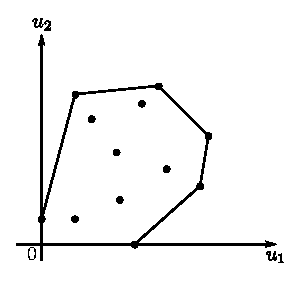
\includegraphics{vol57-figures/fig57-1.eps}}
\end{figure}
\begin{center}
  {\em Newton Polygon of $f$}\\
  (Points of $S_u(f)$ are indicated by dots)
\end{center}

Note that $N_u(f)$ is the set of points $(p_1, p_2) \in \mathbb{R}^2$
for which there exist $(i_1, i_2)$, $(j_1, j_2)$ in $S_u (f)$ and $s,
t \in \mathbb{R}$ with $0 \leq s$, $t \leq 1$ such that 
$$
(p_1 , p_2)= (i_1 st + j_1 (1-s)t, i_2 st + j_2(1-s)t).
$$

\begin{figure}[H]
\centering{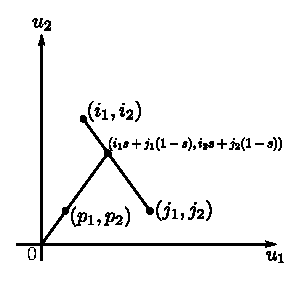
\includegraphics{vol57-figures/fig57-2.eps}}
\end{figure}
We\pageoriginale write $S(f)$ (\resp $N(f)$) for $S_x (f)$ (\resp
$N_x(f)$) and call it simply the {\em support} (\resp {\em Newton
  Polygon})of $f$.

\setcounter{thm}{1}
\begin{thm}\label{part2:chap6:sec19:thm19.2}   
  Let $f$, $g$ be elements of $A$ such that $J(f, g)=
  \diameter$. Assume that $f$ has only one point at infinity and that
  $\deg f \geq 2$. Then there exists an automorphic pair $u= (u_1,
  u_2)$ for $A$ such that $\deg_u f< \deg f$. 
\end{thm}

\begin{proof}
  Let $\ob{k}$ be the algebraic closure of $k$. Since $f$ has only one
  point at infinity, there exists an irreducible homogeneous element
  $F$ in $A$ such that $f^+= \diameter F^n$ for some positive integer
  $n$ and 
\end{proof}

\setcounter{mysubsection}{2}
\subsubsection{}\label{part2:chap6:sec19:sss19.2.1}   
$F$ \textit{is a power of a homogeneous linear polynomial in}
  $\ob{k}[x_1, x_2]$.

Since char $k=0$, the homogeneous polynomial $F$, being irreducible in
$k[x_1, x_2]$, factors into distinct (i.e. mutually coprime)
homogeneous linear polynomials in $\ob{k}[x_1, x_2]$. Therefore in
view of  \ref{part2:chap6:sec19:sss19.2.1}  we necessarily have $\deg
F=1$, so that by a suitable homogeneous linear change of variables in
$A$, we may assume that $F= x_2$ and $f^+ = \diameter x+2^n$ with $n =
\deg f \geq 2$. Then $(0, n) \in S(f)$ and $i_1 + i_2 < n$
for\pageoriginale all $(i_1, i_2)\in S(f)- \{ (0, n)\}$. It follows
that $(0, n) \in N(f)$ and $i_1 + i_2 < n$ for all $(i_1, i_2) \in
N(f)- \{ (0, n) \}$. (this means that $N(f)$ lies below the line
through $(0, n)$ with slope $-1$ and meets that line only in the point
$(0, n)$. See the figure below.) Since $J(f, g)= \diameter$ and $n
\geq 2$, we have $f \notin k[x_2]$. Therefore there exists $(i_1, i_2)
\in S(f)$ with $i_1 > 0$. Let
$$
q= \inf \left\{ (n-i_2) /i_1 \Big| (i_1, i_2) \in S(f), i_1 > 0\right\}
$$
and let $(p_1, p_2)\in S(f)$ be such that $q= (n-p_2)/p_1$. (Note that
$(p_1, p_2)$ is one of 
\begin{figure}[H]
\centering{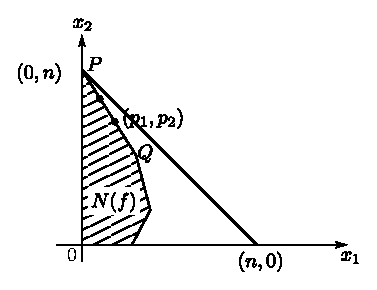
\includegraphics{vol57-figures/fig57-3.eps}}
\end{figure}
the points of $S(f)- \{ (0, n)\}$ lying on the line $PQ$ in the above
figure and that $-q$ is the slope of the line $PQ$.) Let $w= (w_1,
w_2)$, where $w_1 = n- p_2$, $w_2=p_1$. Since $p_1+ p_2< n$, we have
$w_1> w_2$. Therefore by Theorem \ref{part2:chap6:sec18:thm18.13} we
have $f^+_w = \diameter u_1^{r_1}u_2^{r_2}$, where $r_1$, $r_2$ are
non-negative integers with $r_1+ r_2 > 0$, $u_2 = x_2$ and $u_1 =
x_1+ax_2^{w_1/w_2}$ with\pageoriginale $a\in k$ and $w_1/w_2 \in
\mathbb{N}$ if $a \neq 0$. Let $(i_1, i_2)\in S(f)$. Then, since $i_2
\leq n$ and since $q=w_1/w_2$, we get $i_1 w_1 + i_2 w_2\leq
nw_2$. This, together with the fact that $p_1 w_1 + p_2 w_2= nw_2$,
shows that $d_w(f)= nw_2$ and that the two distinct points $(0, n)$
and $(p_1, p_2)$ belong to $S(f^+_w)$. Therefore $f^+_w$ is not a
monomial in $x_1, x_2$. This means that $r_1 \neq 0$ and $a \neq
0$. Therefore by Theorem \ref{part2:chap6:sec18:thm18.13} we have
$\deg_u f < \deg f$, and the theorem is proved.

\begin{remark}\label{part2:chap6:sec19:rem19.2}    
  Let $u= (u_1 , u_2)$ be an automorphic pair for $A$. Let $\sigma$ be
  the $k$-algebra automorphism of $A$ defined by $\sigma (x_i) = u_i$,
  $i=1, 2$. Let us say that $u$ is {\em obtained} from $x$ by
  $\sigma$. We say $\sigma$ is {\em homogeneous linear} if there exist
  $a_i, b_i \in k$ such that $u_i = a_i x_1 + b_i x_2$, $i=1,2$. We
  say $\sigma$ is {\em very primitive} if there exist $a \in k$ and $n
  \in \mathbb{Z}$, $n \geq 2$, such that $u_1 = x_1+ ax_2^n$, $u_2=
  x_2$ or $u_1 = x_1$, $u_2= x_2 + ax_1^n$. We then note from the
  proof of Theorem \ref{part2:chap6:sec19:thm19.2} that there exists
  an automorphic pair $u$ for $A$ such that $\deg_u f< \deg f$ and $u$
  is obtained from $x$ by a homogeneous linear automorphism followed
  by a very primitive automorphism.   
\end{remark}

\begin{thm}\label{part2:chap6:sec19:thm19.4}   
  The following four statements are equivalent:
  \begin{enumerate}[\rm (i)]
  \item If $f, g \in A$ and $J(f, g)= \diameter$ then $k[f, g]=A$.
    \item If $f, g \in A$ and $J (f, g)= \diameter$ then $f$ has only
      one point at infinity.
      \item If $f, g \in A$ and $J(f, g)= \diameter$ then $N(f)$ is a
        triangle with vertices $(0, n)$, $(0, 0)$, $(m, 0)$ for some
        non-negative integers $m$, $n$.
        \item If $f, g \in A$ and $J(f, g)= \diameter$ then $\deg f$
          divides $\deg g$ or $\deg g$ divides $\deg f$.
  \end{enumerate}
\end{thm}

\begin{proof}
~

  (I) $\Rightarrow$ (II). This follows from Corollary
  \ref{part1:chap4:sec11:coro11.24}.

  (II) $\Rightarrow$ (I). If $\deg f \geq 2$ then, since by (II) $f$
  has only one point at infinity,\pageoriginale it follows from
  Theorem \ref{part2:chap6:sec19:thm19.2} that there exists an
  automorphic pair $u= (u_1, u_2)$ for $A$ such that $\deg_u f < \deg
  f$. Moreover, $J_u (f, g)= \diameter$, so that $f$ has only one
  point at infinity with respect to $u$. Therefore, by a repeated
  application of (II) and Theorem \ref{part2:chap6:sec19:thm19.2}, we
  may assume that $\deg f=1$. Now, by a further linear automorphism of
  $A$, we may assume that $f = x_1$. Then $\diameter = J(f, g)= D_2
  (g)$, which shows that $g= \diameter x_2+ p(x_1)$ with $p(x_1) \in
  k[x_1]$. Now, it is clear that $k[f, g]=A$.

  (I) $\Rightarrow$ (III). Let $m= \deg_{x_1} f$, $n= \deg
  _{x_2}f$. Let $T$ be the triangle with vertices $(0, n)$, $(0,0)$,
  $(m, 0)$. We {\em claim} that $N{f}=T$. This is clear if $m=0$ or
  $n=0$. Assume therefore that $m \geq 1$ and $n \geq 1$. Then by
  Corollary \ref{part1:chap4:sec11:coro11.20} $f$ is almost monic in
  both $x_1$ and $x_2$. This means that $(m, 0) \in S(f)$ and $(0,
  n)\in S(f)$. Therefore $T \subset N(f)$. Now, let
  $$
  f= a_0 (x_1) x_2^n + a_1 (x_1) x_2^{n-1} + \cdots + a_n (x_1)
  $$
  with $a_i (x_1) \in k [x_1]$ for $0 \leq i \leq n$. Then by
  Corollary \ref{part1:chap4:sec11:coro11.20} we have $n \deg_{x_1}
  a_i (x_1)\leq im$ for every $i$, $0 \leq i \leq n$. It follows that
  if $(p, q) \in S(f)$ then $n p\leq (n-q)m$, so that $np+mq-mn \geq
  0$. This shows that $(p, q) \in T$. Therefore $S(f) \subset T$ and
  hence $N(f)\subset T$. Thus $N(f) = T$.

  (III) $\Rightarrow$ (II). We may assume that $k$ is algebraically
  closed. Let $d= \deg (f)$. Suppose $f$ has at least two points at
  infinity. Then by a linear homogeneous change of variables (i.e. by
  replacing $x_1, x_2$ by a suitable $k$-basis of $kx_1 \oplus kx_2$)
  we may assume that $f^+= x_!^r G$, where $r$ is a positive integer
  and $G$ is a homogeneous element of $A$ such that $x_1$ does not
  divide $G$ in $A$ and $\deg G >0$. Since $J(f, g)= \diameter$,
  $N(f)$ is a triangle with vertices $(0, n)$, $(0.0)$, $(m, 0)$,
  where\pageoriginale $m, n$ non-negative integers such that $m+n >
  0$. This shows that if $n\geq m$ then the monomial $x_2^n$ appears
  in $f^+$ with a non-zero coefficient. But this is not possible,
  since $f^+= x_1^r G$ with $r>0$. Thus we have $n< m$. Therefore,
  since $N(f)$ is the triangle $(0, n)$, $(0, 0)$, $(m, 0)$, we get
  $f^+ = \diameter x_1^m$. This is also not possible since $x_1$ does
  not divide $G$ and $\deg G> 0$. 

(I) $\Rightarrow$ (IV). This follows from
  Theorem \ref{part1:chap4:sec10:thm10.2}.

(IV) $\Rightarrow$ (I). Assuming (IV), we prove (I) by induction on
  $\deg (fg)$. Since $J(f, g)= \diameter$, we have $f \notin k$, $g
  \notin k$. Therefore $\deg f \geq 1$, $\deg g\geq 1$ and $\deg(fg)
  \geq 2$. If $\deg (fg) =2$ then $\deg f=1= \deg g$ and the assertion
  is clear in this case. Now, let $m= deg f$, $n = \deg g$, and assume
  that $m+n \geq 3$. Without loss of generality, we may assume that $m
  \geq n$. Then by (IV) $n$ divides $m$. Since $\deg (fg) \geq 3$ and
  $J(f, g)= \diameter$, we have $J(f^+ , g^+)=0$ by Lemma
  \ref{part2:chap6:sec18:lem18.2}. Therefore by Proposition
  \ref{part2:chap6:sec17:prop17.4} we have $f^+= c(g^+)^{m/n}$ for
  some $c \in k^*$. Let $h= f- cg^{m/n}$. Then $\deg h < \deg
  f$. Moreover, clearly $J(h, g)= J(f, g)= \diameter$. Therefore
  $k[h,g]=A$ by induction hypothesis. Since $k[f, g]= k[h, g]$, (I)
  is proved.
\end{proof}

\begin{remark}\label{part2:chap6:sec19:rem19.5}
  In order to solve the Jacobian problem, we may assume that the field
  $k$ is algebraically closed. For, each of statements (II), (III) and
  (IV) of Theorem \ref{part2:chap6:sec19:thm19.4} is unaltered if we
  replace $k$ by its algebraic closure.
\end{remark}

\begin{remark}\label{part2:chap6:sec19:rem19.6}
  In the next section we give yet another equivalent formulation of
  the Jacobian problem in terms of a Newton-Puiseux expansion.
\end{remark}

\section{Jacobian Problem Via Newton-Puiseux
  Expansion}\label{part2:chap6:sec20} 

We preserve the notation of \S \ref{part2:chap6:sec15} and
\S \ref{part2:chap6:sec16}. In particular, we have char $k=0$. We
assume, in addition, that $k$ is algebraically closed.

\subsection{Newton-Puiseux Expansion}\label{part2:chap6:sec20:ss20.1} 

Let\pageoriginale $f$, $g$ be elements of $A$. Assume that $n=
\deg_{x_2} f > 0$ and that $f$ is monic in $x_2$. By a construction
analogous to the one used in \S \ref{part1:chap4:sec9}, we can expand
$g$ in fractional powers of $f^{-1}$ with coefficients in the algebraic
closure of $k(x_1)$. Explicitly, let $L$ be the algebraic closure of
$k(x_1)$ and let $\tau$ be an indeterminate. Let $\theta: L[x_2]\to L
((\tau))$ be the $L$-algebra monomorphism defined by $\theta (x_2)=
\tau^{-1}$. It is then clear that we have $\ord_\tau \theta (F)= -
\deg_{x_2} F$ for every $F\in L [x_2]$. In particular, we have
$\ord_\tau \theta (f)=- n$. By Corollary
\ref{part1:chap2:sec5:coro5.4} there exists $t \in L ((\tau))$ such
that $\ord_\tau (t) =1$ and $\theta (f) = t^{-n}$. We then have
$L((t))= L((\tau))$ and $\ord_\tau F = \ord_\tau F$ for every $F \in L
((t))$. Let $B= k[x_1]$. Then $B \subset L$ and we have $A=
B[x_2]$. Let 
$$
B((t))= \left\{ \sum a_i t^i \in L ((t)) \Big| a_i \in B \;\;  \forall i \right\}.
$$ 

Then we have

\setcounter{mysubsection}{1}
\subsubsection{LEMMA}\label{part2:chap6:sec20:sss20.1.1} 
$$
\theta (A) \subset B((t)).
$$

\begin{proof}
  We have only to show that $\theta (x_2)= \tau^{-1}$ belongs to
  $B((t))$. Since $f$ is monic in $x_2$ with $\deg_{x_2} f=n$, we can
  write $f= x_2^n+ f_1$ with $f_1 \in A$ and $\deg_{x_2} f_1 <
  n$. Therefore we get
  $$
  t^{-n} = \theta (f) = \tau^{-n} (1+ \tau p)
  $$
  with $p \in B[[\tau]]$. It follows that $t= \zeta \tau(1+\tau q)$,
  where $\zeta \in \mu_n (k)$ ($= n^{\rm th}$ roots of unity in $k$) and 
$$
q \sum_{i=1}^\infty \binom{s}{i} \tau^{i-1} p^i \in B \in B[[\tau]].
 $$
where $s=- 1/n$. Replacing $t$ by $\zeta^{-1} t$, we may assume that
$\zeta =1$. Let $\tau = \displaystyle{\sum_{i=1}^\infty} a_i t^i$\pageoriginale with
$a_i \in L$. Then we get
$$
\tau = \sum^\infty_{i=1} a_i \tau^i (1 + \tau_q)^i.
$$
Now, we can write $(1 +  \tau q)^i= 1+ \tau q_i$ with $q_i \in B
[[\tau]]$. Let $q_i = \displaystyle{\sum^\infty_{j=0}}b_{ij} \tau^j$
with $b_{ij} \in B$. Then we get
\begin{equation*}
  \tau = \sum^\infty_{i=1} a_i \tau^i \left(1+ \sum^\infty_{j=0}
  b_{ij} \tau^{j+1}\right). \tag{20.1.1.1}\label{part2:chap6:sec20:eq20.1.1.1} 
\end{equation*}
Comparing the coefficients of $\tau$, we get $a_1 = 1 \in
B$. Inductively, assume that $a_i \in B$ for $ 1 \leq i \leq d -1$ for
some integer $d \geq 2$. Then, comparing the coefficients of $\tau^d$
in (\ref{part2:chap6:sec20:eq20.1.1.1}) we get $0= a_d+c$, where
$$
c= \sum_{i=1}^{d-1} a_i b_{i, d-1-i}.
$$
By induction hypothesis $c \in B$. Therefore $a_d \in B$. This proves
that we have 
\begin{equation*}
  \tau = t(1+ \tr)\tag{20.1.1.2}\label{part2:chap6:sec20:eq20.1.1.2} 
\end{equation*}
with $r \in B [[t]]$. Therefore we get
$$
\tau^{-1} = t^{-1} \left(1+ \sum^\infty_{i=1} (-1)^i t^i r^i \right).
$$
which shows that $\tau^{-1} \in B ((t))$.
\end{proof}


\subsubsection{COROLLARY}\label{part2:chap6:sec20:sss20.1.2}

For any choice of $t \in L ((\tau))$ such that $\theta (f) = t^{-n}$,
we have $\tau = \zeta t(1+ \tr)$ for some $r \in B[[t]]$ and some
$\zeta \in \mu_n (k)$.


\begin{proof}
  Immediate from (\ref{part2:chap6:sec20:eq20.1.1.2}).

In view of Lemma \ref{part2:chap6:sec20:sss20.1.1}, we can restrict
$\theta$ to $A$ to get a $B$-algebra monomorphism $\theta: A \to
B((t))$ such that $\theta (f) = t^{-n}$ and 
\begin{equation*}
  \ord_t \theta (F) =- \deg_{x_2} F
  \tag{20.1.3}\label{part2:chap6:sec20:eq20.1.3} 
\end{equation*}
for\pageoriginale every $F \in A$. Let
\begin{equation*}
  \theta (g) = \sum_j g_j t^j \tag{20.1.4}\label{part2:chap6:sec20:eq20.1.4} 
\end{equation*}
with $g_j = g_j (x_1) \in B$. We call
(\ref{part2:chap6:sec20:eq20.1.4}) a {\em Newcon-Puiseux expansion of
  $g$ in fractional powers of $f^{-1}$}. Note that for fixed $x_1,
x_2, f, g$, (\ref{part2:chap6:sec20:eq20.1.4}) depends on the choice
of an element $t$ such that $\theta (f)= t^{-n}$. If $t_1$, $t_2$ are
two such choices then we have $t_1 = \zeta t_2$ for some $\zeta \in
\mu_n (k)$. Thus there are atmost $n$ distinct Newton-Puiseux
expansions of $g$ in fractional powers of $f^{-1}$ and any two of
them are conjugate to each other under a $B$-automorphism of $B((t))$
given by $t \mapsto \zeta t$ for some $\zeta \in \mu_n (k)$. In
particular, the condition (JC) in
Definition \ref{part2:chap6:sec20:def20.2} below depends only on $x=
(x_1, x_2)$, $f$, $g$ and does not depend upon $t$.
\end{proof}

\setcounter{thm}{1}
\begin{defi}\label{part2:chap6:sec20:def20.2} 
  With the notation of \ref{part2:chap6:sec20:ss20.1}, we say the pair
  $(f, g)$ {\em satisfies condition $(JC)$ (with respect to $X$)} if the
  following holds:

  $(JC) \; g_j \in k$ {\em for every} $j \leq n-2$ {\em and} $\deg_{x_1}
  g_{n-1}=1$. 
\end{defi}

\setcounter{subsection}{2}
\subsection{A DERIVATION OF $L((t))$.}\label{part2:chap6:sec20:ss20.3}

Continuing with the notation of \ref{part2:chap6:sec20:ss20.1}, put
$u_1 = x_1$, $u_2 = f$ and $u= (u_1, u_2)$. Since $\deg_{x_2} f> 0$,
$u$ is a transcendence base of $K=k(x_1, x_2)$ over $k$. Therefore we
have $k$-derivations $D_{u, 1}, u_{u, 2}$ of $K$ as defined
in \ref{part2:chap6:sec15:ss15.1}. Let $d_i$ denote the unique
extension of $D_{u, i}$ to a $k$-derivation of $L(x_2)$, $i = 1,
2$. Let $\delta : L((t)) \to L ((t))$ be the map defined by 
$$
\delta \left( \sum_j a_j t^i \right) = \sum_j d_1 (a_j) t^j.
$$
 
Then $\delta$ is clearly a $k((t))$-derivation of $L((t))$. We note
that $\delta (B((t))) \subset B((t))$.

Moreover,\pageoriginale denoting again by $\theta$ the extension of
$\theta$ to an $L$ - monomorphism $L(x_2) \to L((t))$ of fields, we have

\setcounter{mysubsection}{3}
\subsubsection{LEMMA}\label{part2:chap6:sec20:sss20.3.1}
$$
\delta \theta = \theta d_1.
$$

\begin{proof}
  Since $L(x_2)$ is separable algebraic over $k(u_1, u_2)$, it is
  enough to show that $\delta \theta | k(u_1, u_2)= \theta d_1| k(u_1,
  u_2)$. Therefore it is enough to check that $\delta \theta (u_i) =
  \theta d_1 (u_i)$, $i= 1, 2$. Now, $\delta \theta (u_1)= \delta
  \theta (x_1)= \delta (x_1)= \delta(u_1)=1$ and $\theta d_1 (u_1)=
  \theta (1) =1$. Next, $\delta \theta (u_2)= \delta \theta(f)= \delta
  (t^{-n})=0$ and $\theta d_1 (u_2) = \theta (0) =0$. The lemma is proved.
\end{proof}

\setcounter{thm}{3}
\begin{thm}\label{part2:chap6:sec20:thm20.4}
  Let $f$, $g$ be elements of $A$. Assume that $f$ is monic in $x_2$
  and that $\deg_{x_2} f> 0$. Then the following two conditions are
  equivalent:
\begin{enumerate}[\rm (i)]
\item $J(f, g)=\diameter$.
\item $(f, g)$ satisfies $(JC)$.
\end{enumerate}
\end{thm}

\begin{proof}
  We use the notation of \ref{part2:chap6:sec20:ss20.1}
  and \ref{part2:chap6:sec20:ss20.3}. Let $D_i = D_{x. i}, i=1,2$,
  where $x= (x_1, x_2)$. By the chain rule of derivation we have
\begin{align*}
  J(f, g) & = J_u (f, g) J_x (u_1, u_2)\\
  & = J_u (f, g) J_x (x_1, f)\\
  & = \det \begin{pmatrix}
    0 & 1\\ 
d_1 (g) & d_2 (g)
  \end{pmatrix}\det
  \begin{pmatrix}
    1 & 0\\ 
D_1 (f) & D_2 (f)
  \end{pmatrix}\\
  & = -d_1(g) D_2 (f).
\end{align*}
This gives 
$$\theta (d_1 (g)) \theta (D_2 (f))= - \theta (J (f, g)).$$ 
Therefore by Lemma~\ref{part2:chap6:sec20:sss20.3.1} we get
$\delta (\theta (g)) \theta (D_2 (f))= - \theta (J (f, g))$. Using the
expression (\ref{part2:chap6:sec20:eq20.1.4}) for $\theta (g)$ we get 
\begin{equation*}
\left( \sum_j d_1 (g_j) t^i\right) \theta (D_2 (f))= -\theta (J (f,
g)).\tag{20.4.1}\label{part2:chap6:sec20:eq20.4.1} 
\end{equation*}

Now,\pageoriginale let $n= \deg_{x_2}f$. Then $n \geq 1$. Since $f$ is
monic in $x_2$, we get $D_2(f)= n x_2^{n-1}+ f'$ with $f' \in A$ and
$\deg_{x_2}f'< n-1$. Therefore $\theta (D_2 (f))= n \tau^{1-n}+ \theta
(f')$ with $\ord_\tau \theta (f') > 1-n$. It therefore follows from
Corollary \ref{part2:chap6:sec20:sss20.1.2} that $\theta (D_2 (f))=
\diameter t^{1-n}+e$, where $e \in L ((t))$ and $\ord_t e> 1-n$. This
shows that we have $\theta (D_2 (f))^{-1}= \diameter t^{n-1} + h$ with
$h \in L ((t))$ and $\ord_t h > n-1$. Therefore
from (\ref{part2:chap6:sec20:eq20.4.1})  we get
\begin{equation*}
  \sum_j d_1 (g_j)t^j =- \theta (J(f, g)) (\diameter t^{n-1} +
  h).\tag{20.4.2} \label{part2:chap6:sec20:eq20.4.2} 
\end{equation*}
Now, suppose $J(f, g)=\diameter$. Then we have
$$
\sum_j d_1 (g_j) t^j = \diameter (\diameter t^{n-1} + h).
$$
This shows that $d_1 (g_j)=0$ for $j \leq n-2$ and $d_1 (g_{n-1})=
\diameter$, which clearly implies that $(f, g)$ satisfies condition
$(JC)$.

Conversely, suppose that $(f, g)$ satisfies condition $(JC)$. Then we
have $d_1 (g_j)=0$ for $j \leq n-2$ and $d_1 (g_{n-1})=
\diameter$. Therefore it follows from
(\ref{part2:chap6:sec20:eq20.4.2}) that we have
\begin{equation*}
  \diameter t^{n-1}+ \sum_{j \leq n} d_1 (g_j)t^j=- \theta (J(f, g))
  (\diameter t^{n-1}+ h).\tag{20.4.3}\label{part2:chap6:sec20:eq20.4.3} 
\end{equation*}
This shows that $\ord_t \theta (J(f, g))=0$. Therefore by
(\ref{part2:chap6:sec20:eq20.1.3}) we get $\deg_{x_2}$ $J (f, g)=0$,
which means that $J(f, g)\in L$. Put $\lambda = J(f, g)$. Then $\theta
(\lambda)= \lambda$. Therefore comparing the coefficients of $t^{n-1}$
in (\ref{part2:chap6:sec20:eq20.4.3}) we get $\diameter =- \lambda
\diameter$, which shows that $\lambda = \diameter$, and the theorem is proved.
\end{proof}

\begin{notn}\label{part2:chap6:sec20:notn20.5}
  Let $f, g$ be elements of $A$. Assume that $n= \deg_{x_2}\break f > 0$ and
  that $f$ is monic in $x_2$. Then with the notation of
  \ref{part2:chap6:sec20:ss20.1} we have a commutative diagram

\[
\xymatrix{L[x_2] \ar[r]^\theta & L((t))\\
A \ar@{^{(}->}[u] \ar[r]^\theta & B((t))\ar@{^{(}->}[u]
}
\]  
where\pageoriginale $\theta$ is a $B$-algebra monomorphism such that
$\theta (f)= t^{-n}$ and 
\begin{equation*}
  \ord_{t}\theta (F) = - \deg_{x_2}F
  \tag{20.5.1} \label{part2:chap6:sec20:eq20.5.1} 
\end{equation*}
for every $F \in A$. Let
$$
\theta (g) = \sum_j g_j t^i
$$
with $g_j= g_j (x_1) \in B$. {\em Assume that the pair $(f, g)$ satisfies
condition (JC), i.e. assume that we have}
\begin{equation*}
\begin{aligned}
  & g_j \in k \text{ for every } j \leq n-2,\\
  & \deg_{x_1} g_{n-1}=1.
\end{aligned}\tag{20.5.2}\label{part2:chap6:sec20:eq20.5.2}
\end{equation*}
Then by Theorem \ref{part2:chap6:sec20:thm20.4} we have $J(f, g)=
\diameter$. Let $\tilde{\Phi}= \tilde{\Phi} (X, Y)\in L((X))[Y]$ be
the minimal monic polynomial of $\theta (g)$ over $L((t^n))$. (See
Definition \ref{part1:chap2:sec5:def5.8}.) Recall that $\tilde{\Phi}$
is the unique irreducible element of $L((X)) [Y]$, monic in $Y$, such
that $\tilde{\Phi} (t^n, \theta (g))=0$. Put $\Phi = \Phi (X, Y)= \tilde{\Phi}
(X^{-1}, Y)$.
\end{notn}

\setcounter{mysubsection}{5}
\setcounter{subsubsection}{2}
\subsubsection{LEMMA}\label{part2:chap6:sec20:sss20.5.3}
\begin{enumerate}[(i)]
\item $\Phi$ is monic in $Y$ and $\deg_Y \Phi=n$.
  \item $\Phi \in B [X, Y]$.
    \item $\Phi (f, g)=0$.
      \item $L [X, Y]/(\Phi)$ is isomorphic (as an $L$-algebra) to
        $L[f, g]$.
\end{enumerate}

\begin{proof}
  ~
  \begin{enumerate}[(i)]
    \item By definition of $\Phi$, $\Phi$ is monic in $Y$. By
      (\ref{part2:chap6:sec20:eq20.5.2}) $n-1 \in \Supp_t \theta
      (g)$. Therefore
      $$
      \text{\gcd}~ ( \{ n\} \cup \Supp_t \theta (g))=1.
      $$
      Now\pageoriginale it follows from Lemma \ref{part1:chap2:sec5:lem5.10} that
     $\deg_Y \tilde{\Phi} =n$. This proves (i).
      \item Let $\Psi = \Psi (X, Y) \in B [X, Y]$ be the
        $x_2$-resultant of $(f- X, Y-g)$. Since $f$ is monic in $x_2$,
        $\Psi$ is monic in $Y$. Moreover, since $\deg_{x_2} f=n$, we
        have $\deg_Y \Psi =n$. Put $\tilde{\Psi} (X, Y)= \Psi (X^{-1},
        Y)$. We have $\Psi (f, g)=0$. Therefore $0 = \theta (\Psi (f,
        g))= \Psi (t^{-n} , \theta (g))= \tilde{\Psi} (t^n , \theta
        (g))$. It now follows from (i) that $\tilde{\Phi} =
        \tilde{\Psi}$. Therefore $\Phi = \Psi \in B [X, Y]$.
        \item Since $\Phi= \Psi$ as proved above, we have $\Phi (f,
          g)= \Psi (f, g)=0$.
          \item Let $\alpha: L [X, Y] \to L[f, g]$ be the $L$-algebra
            epimorphism defined by $\alpha(X) = f$,
            $\alpha(Y)=g$. then (ii) and (iii) $\Phi \in \ker
            \alpha$. Since $\Phi$ is irreducible in $L((X^{-1})) [Y] \supset
            L[X, Y]$ and is monic in $Y$, $\Phi$ is irreducible in $L[X,Y]$. Therefore $\ker \alpha = (\Phi)$, and (iv) is proved.
  \end{enumerate}
\end{proof}

\subsubsection{A SPECIALIZATION.} \label{part2:chap6:sec20:sss20.5.4}

Since $\deg_{x_1}g_{n-1}= 1$ by (\ref{part2:chap6:sec20:eq20.5.2}),
there exists $c \in k$ such that $g_{n-1} (x_1)\neq g_{n-1}(c) \neq
0$. We choose such a $c \in k$ and keep it fixed in the sequel. For an
element $F$ of $A= B[x_2]$ (\resp $B((t))$, $B[X, Y]$, $B[X^{-1}, Y],
\ldots $) we shall denote by $\ob{F}$ the element of $k[x_2]$ (\resp
$k((t))$, $k[X, Y]$, $k[X^{-1}, Y], \ldots$) obtained from $F$ by
putting $x_1=c$. Let $\varphi= \tilde{\Phi}$, $\tilde{\varphi} =
\ob{\tilde{\Phi}}$.

\subsubsection{LEMMA}\label{part2:chap6:sec20:sss20.5.5}
\begin{enumerate}[(i)]
\item $\varphi \in k[X, Y]$, $\varphi$ is monic in $Y$ and $\deg_Y
  \varphi=n$.
  \item $\tilde{\varphi} \in k [X^{-1}, Y]$ $\tilde{\varphi}$ is monic
    in $Y$ and $\deg_Y \tilde{\varphi} =n$.
    \item $\tilde{\varphi}$ is the minimal monic polynomial of
      $\ob{\theta(g)}= \sum\limits_j \ob{g}_j t^j$ over $k((t^n))$.
      \item $\ord_t (\theta(g)- \ob{\theta (g)})= n-1$.
\end{enumerate}

\begin{proof}
  ~
\begin{enumerate}[(i)]
\item is immediate from Lemma \ref{part2:chap6:sec20:sss20.5.3}.
\item This follows from (i), since $\tilde{\varphi} (X, Y)=
  \varphi(X^{-1}, Y)$.
  \item Since\pageoriginale $\tilde{\Phi} (t^n , \theta (g))=0$, we
    have $\tilde{\varphi} (t^n, \ob{\theta(g)})=0$. Since
    $\ob{g}_{n-1}\neq 0$, we have $n- 1 \in \Supp_t
    \ob{\theta(g)}$. Therefore the minimal monic polynomial of
    $\ob{\theta (g)}$ over $k((t^n))$ has $Y$-degree $n$ (Lemma
    \ref{part1:chap2:sec5:lem5.10}). Therefore by (ii)
    $\tilde{\varphi}$ is the minimal monic polynomial of
    $\ob{\theta(g)}$ over $k((t^n))$.

\item Since $g_j \in k$ for $j \leq n-2$, we have $g_j= \ob{g}_j$ for
  $j \leq n-2$. Moreover, we have $g_{n-1} \neq
  \ob{g}_{n-1}$. Therefore the assertion follows.
\end{enumerate}
\end{proof}

\subsubsection{Characteristic Sequences of $(f,
  g)$.}\label{part2:chap6:sec20:sss20.5.6} 

(See \S\ \ref{part1:chap2:sec6}.) We define $h(f, g)= h(\tilde{\Phi})$
and we define the {\em characteristic sequences} of the pair $(f, g)$
by 
\begin{align*}
  m_i (f, g)& = m_i (-n, \tilde{\Phi}),\\
  q_i(f, g) & = q_i (-n, \tilde{\Phi}),\\
  s_i (f, g) & = s_i (-n, \tilde{\Phi}),\\
  r_i (f, g) & = r_i (-n, \tilde{\Phi}),\\
   d_{i+1}(f, g) & = d_{i+1} (\tilde{\Phi}),
\end{align*}
for $0 \leq i\leq h (f, g)+1$. (Note that these sequences depend not only
on $f$, $g$, but also on $x= (x_1, x_2)$. However, the omission of
$x$ in the notation $m_i (f, g)$ etc. will cause no confusion.)

\subsubsection{LEMMA}\label{part2:chap6:sec20:sss20.5.7}

We have  $h(\tilde{\varphi}) = h(f, g)$ and 
\begin{align*}
  m_i (-n, \tilde{\varphi}) & = m_i (f, g),\\
  q_i (-n, \tilde{\varphi}) & = q_i (f, g),\\
  s_i (-n, \tilde{\varphi}) & = s_i (f, g),\\
  r_i (-n, \tilde{\varphi}) & = r_i (f, g),\\
  d_{i+1} (\tilde{\varphi}) & = d_{i+1} (f, g)
\end{align*}
for $0 \leq i \leq h (\tilde{\varphi})+1$.

\begin{proof}
  Immediate,\pageoriginale since \gcd $(n, n-1)= 1$, $n-1 \in \Supp_t
  \ob{\theta(g)}$, $n-1 \in \Supp_t \theta (g)$ and $\ord_t (\theta
  (g) - \ob{\theta(g)})= n-1$ by Lemma \ref{part2:chap6:sec20:sss20.5.5}. 
\end{proof}

{\em In the remainder of subsection \ref{part2:chap6:sec20:notn20.5}
  we fix the following notation:}
\begin{align*}
  h & = h(f, g),\\
  m_i & = m_i (f, g),\\
  q_i & = q_i (f, g),\\
  s_i & = s_i (f,g),\\
r_i & = r_i (f,g),\\
  d_{i+1} & = d_{i+1} (f, g)
\end{align*}
for $0 \leq i \leq h+1$. Also, for $1 \leq i \leq h+1$, let
\begin{align*}
  \tilde{\psi}_i & = 
  \begin{cases}
    Y, & \text{if}~ i=1,\\
    App_Y^{d_i} (\tilde{\psi}, & \text{if}~ i \geq 2
  \end{cases}\\
  \psi_i & =
  \begin{cases}
    Y, & \text{if}~ i \geq 1,\\
    App_Y^{d_i}(\varphi), & \text{if}~ i \geq 2,
  \end{cases}\\
  \tilde{\psi'}_i & = \frac{\partial \tilde{\psi} i}{\partial Y},\\
  \psi'_i & = \frac{\partial \psi_i}{\partial Y}.
\end{align*}
(See \S\ \ref{part1:chap1:sec4}).

\subsubsection{LEMMA}\label{part2:chap6:sec20:sss20.5.8}

We have:
\begin{enumerate}[(i)]
\item $h \geq 1$.
\item $m_1 =  - \deg_{x_2}g \leq 0$.
\item $m_i < n-1$ for $1 \leq i \leq h-1$ and $m_h \leq n-1$.
\end{enumerate}

\begin{proof}
\begin{enumerate}[(i)]
\item This\pageoriginale is clear, since $\theta (g)\neq 0$.
\item Follows from (\ref{part2:chap6:sec20:eq20.5.1}) and the fact
  that $g \neq 0$.
  \item This is also clear, since $n-1 \in \Supp_t \theta (g)$ and
    \gcd $(n, n-1)=1$.
\end{enumerate}
\end{proof}

\subsubsection{LEMMA}\label{part2:chap6:sec20:sss20.5.9}

For $1 \leq i \leq h+1$, we have
\begin{enumerate}[(i)]
\item $\tilde{\psi}_i (X, Y)= \psi_i (X^{-1}, Y)$,
  \item $\tilde{\psi'}_i (X, Y)= \psi'_i (X^{-1}, Y)$.
\end{enumerate}

\begin{proof}
\begin{enumerate}[(i)]
\item Follows from Proposition \ref{part1:chap1:sec4:prop4.7}.
\item Follows from (i)
\end{enumerate}
\end{proof}

\subsubsection{LEMMA}\label{part2:chap6:sec20:sss20.5.10}

For $F(X, Y) \in k[X, Y]$, we have $\deg_{x_2} F(f, g)= - \ord_t
F(t^{-n}, \theta (g))$.

\begin{proof}
  This follows from \ref{part2:chap6:sec20:eq20.5.1}, since
  $\theta(F(f, g))= F(t^{-n}, \theta (g))$.  
\end{proof}

\subsubsection{LEMMA} \label{part2:chap6:sec20:sss20.5.11}

For $1 \leq e \leq h$, we have $\deg_{x_2} \psi_e (f, g)= - r_e$.

\begin{proof}
  We have $\psi_1 (X, Y)= Y$. Therefore by
  Lemma \ref{part2:chap6:sec20:sss20.5.10} $\deg_{x_2} \psi_1$ $(f, g)=
  - \ord_t \theta (g) =- m_1= - r_1$. This proves the assertion for
  $e=1$. Assume now that $e \geq 2$. Since $m_e \leq n-1$ by
  Lemma \ref{part2:chap6:sec20:sss20.5.8}, it follows from Lemma
  \ref{part2:chap6:sec20:sss20.5.5} (iv) that we have
$$
\theta (g) = \sum_{j < m_e} \ob{g}_j t^j + g_{m_e} t^{m_e} + \sum_{j >
  m_e} g_j t^j.
$$
Therefore, since $g_{m_e} \neq 0$, it follows from
Corollary \ref{part1:chap3:sec7:coro7.20} that \break $\ord_t \tilde{\psi}
(t^n, \theta(g))= r_e$. Therefore by Lemma
\ref{part2:chap6:sec20:sss20.5.9} we have $\ord_t \psi_e (t^{-n}$,
 $\theta (g))= r_e$. Now, the lemme follows from Lemma
\ref{part2:chap6:sec20:sss20.5.10}. 
\end{proof}

\subsubsection{LEMMA}\label{part2:chap6:sec20:sss20.5.12}

For $1 \leq e \leq h$, we have $\deg_{x_2} \psi'_e (f, g)= m_e - r_e$.

\begin{proof}
  Since $\ord_t (\theta(g)- \ob{\theta(g)})= n-1 \geq m_e$ and $m_e
  \in \Supp_t \theta (g)$, it follows from
  Proposition \ref{part1:chap5:sec13:prop13.7} that $\ord_t
  \tilde{\psi'}_e (t^n, \theta (g))= r_e - m_e$. Therefore by Lemmas
  \ref{part2:chap6:sec20:sss20.5.9} and
  \ref{part2:chap6:sec20:sss20.5.10} we get $\deg_{x_2} \psi'_e (f,
  g)=- \ord_t$ $\psi'_e (t^{-n}, \theta (g))= m_e - r_e$. 
\end{proof}


\begin{defi}\label{part2:chap6:sec20:def20.6}
 An\pageoriginale element $f$ of $A$ is said to be $x_2$ {\em regular}
 if $f \neq 0$ and $\deg f = \deg_{x_2} f$.
\end{defi}

Note that $f$ is $x_2$-regular if and only of $x_1$ does not divide
$f^+$ in $A$.

In Lemmas \ref{part2:chap6:sec20:lem20.7} -
\ref{part2:chap6:sec20:lem20.9} below, we let the notation and
assumptions be those \ref{part2:chap6:sec20:notn20.5}. We assume,
moreover, that $f$ ix $x_2$-regular.

\begin{lemma}\label{part2:chap6:sec20:lem20.7}
  Let $e$ be an integer, $2 \leq e \leq h$. Assume that $\psi_i (f,
  g)$ is related to $f$ for every $i$, $1 \leq i \leq e-1$. Let $F=
  F(X, Y)$ be a non-zero element of $k[X, Y]$ with $\deg_Y F<
  n/d_e$. Then $F(F, g)$ is related to $f$.
\end{lemma}

\begin{proof}
  Let $R = k[X]$. Let $p= e-1$ and let $G= (G_1 , \ldots , G_p)$,
  where $G_i = \psi_i$ for $1 \leq i \leq p$. Then $G$ satisfies
  conditions (i)-(iii) of \ref{part1:chap1:sec2:ss2.2} and, with the
  notation of \ref{part1:chap1:sec2:ss2.2}, we have $n_i (G) = d_i
  /d_{i+1}$ for $1 \leq i \leq  p-1$. Let
  $$ 
  A(G)=\left\{ a = (a_1, \ldots , a_p) \in (\mathbb{Z}^+)^p \Big| a_i
  < d_i/ d_{i+1} ~\text{for}~ 1 \leq i \leq p-1\right\}.
  $$
\end{proof}

Then by Corollary \ref{part1:chap1:sec2:coro2.14} we have the $G$-adic
expansion 
\begin{equation*}
  F = \sum_{a \in A(G)} F_a G^a
  \tag{20.7.1}\label{part2:chap6:sec20:eq20.7.1} 
\end{equation*}
of $F$ with $f_a= F_a(X) \in R$ for every $a \in A(G)$. By Corollary
\ref{part1:chap1:sec2:coro2.9} we have
$$
\sum_{i=1}^p a_i \deg_Y G_i = \deg_Y G^a \leq \deg_Y F< n/d_e = n/d_{p+1}
$$
for every $a \in \Supp_G {F}$. In particular, we have
$$
a_p n/d_p= a_p \deg_Y G_p < n/d_{p+1}.
$$

This gives
\begin{equation*}
  a_p < d_p /d_{p+1} \tag{20.7.2}\label{part2:chap6:sec20:eq20.7.2} 
\end{equation*}
for\pageoriginale every $a \in \Supp_G (F)$. Putting $X=f$, $Y=g$
in (\ref{part2:chap6:sec20:eq20.7.1}), we get
\begin{equation*}
  F(f, g) = \sum\limits_{a \in S} F_a (f) G(f, g)^a,
  \tag{20.7.3}\label{part2:chap6:sec20:eq20.7.3}  
\end{equation*}
where $S = \Supp_G (F)$. Since $G_a (f) \in k [f]$, we can rewrite
(\ref{part2:chap6:sec20:eq20.7.3}) in the form 
$$
F(f, g)= \sum_{b \in B(H)} \lambda_b H^b
$$
with $\lambda_b \in k$ for every $b$, where $h= (h_0, \ldots , h_p)$
with $h_0 = f$. $H_i = G_i (f, g)$ for $1 \leq i \leq p$, and where
$$
B(H) = \left\{ b= (b_0 , \ldots , b_p) \in (\mathbb{Z}^+)^{p+1} \Big|
b_i < d_i /d_{i+1} ~\text{for}~ 1 \leq i \leq p\right\}.
$$

Note that the condition $b_p < d_p /d_{p+1}$ for $b \in B(H)$ is
justified in view of (\ref{part2:chap6:sec20:eq20.7.2}). Since
$\deg_{x_2} H_i =- r_i$ for $1 \leq i \leq p$
(Lemma \ref{part2:chap6:sec20:sss20.5.11}) and $\deg_{x_2} H_0 =
\deg_{x_2} f= n=- r_0$, we have, for every $b \in (B(H))$.
$$
\deg_{x_2} H^b= \sum_{i=0}^p b_i (- r_i).
$$
which is clearly a strict linear combination of $(- r_0, \ldots ,
-r_p)$. (See \S\ \ref{part1:chap1:sec1}.) Therefore if $b, b' \in
B(H)$, $b \neq b'$, then $\deg_{x_2} H^b \neq \deg_{x_2} H^{b'}$. It
follows that there exists a unique $b \in B(H)$ such that $\lambda_b
\neq 0$ and 
\begin{equation*}
  \deg_{x_2} F(f, g)= \deg_{x_2} (\lambda_b H^b)> \deg_{x_2}
  (\lambda_{b'} H^{b'})\tag{20.7.4}\label{part2:chap6:sec20:eq20.7.4}
\end{equation*}
for every $b' \in B(H)$, $b' \neq b$. Now, by assumption, $H_i$ is
related to $f$ for every $i$, $0 \leq i \leq p$. In particular, since
$f$ is $x_2$-regular, so is $H_i$ for every $i$, $0 \leq i \leq
p$. Therefore we have $\deg_{x_2} H^{b'}= \deg H^{b'}$ for every $b'
\in B(H)$, and it follows from (\ref{part2:chap6:sec20:eq20.7.4}) that
we have
$$
F(f, g)^+= (\lambda_b H^b).
$$

Since\pageoriginale each $H_i$ is related to $f$, so is $\lambda_b
H^b$ by Lemma \ref{part2:chap6:sec17:lem17.3}. Thus $F(f, g)$ is
related to $f$, and the lemma is proved. 

\begin{lemma}\label{part2:chap6:sec20:lem20.8}
  Let $e$ be an integer, $2 \leq e \leq h$. Assume that $\psi_i (f,
  g)$ is related to $f$ for every $i$, $1 \leq i \leq e-1$. Then $f$
  has only one point at infinity or $\psi_e (f, g)$ is $x_2$-regular.
\end{lemma}

\begin{proof}
  By the chain rule for differentiation we have
\begin{equation*}
  J(f, \psi_e (f, g))= \psi'_e (f, g) J (f, g)= \diameter \psi'_e (f,
  g). \tag{20.8.1} \label{part2:chap6:sec20:eq20.8.1}
\end{equation*}
Now, if $J(f^+, \psi_e (f, g)^+)=0$ then by
Proposition \ref{part2:chap6:sec17:prop17.4} $f$ and $\psi_e (f, g)$
are related. Therefore in this case, since $f$ is $x_2$-regular, so is
$\psi_e(f, g)$. Thus we may now assume that $J(f^+, \psi_e (f,
g)^+)\neq 0$. Then by (\ref{part2:chap6:sec20:eq20.8.1}) and
Lemma \ref{part2:chap6:sec18:lem18.2} we have
\begin{equation*}
  J(f^+, \psi_e (f, g)^+) = \diameter \psi'_e (f,
  g)^+. \tag{20.8.2} \label{part2:chap6:sec18:eq20.8.2} 
\end{equation*}
\end{proof}

Since $\deg_Y \psi'_e= \deg_Y \psi_e -1 < n/d_e$, it follows from
Lemma \ref{part2:chap6:sec20:lem20.7} that $\psi'_e (f, g)$ is related
to $f$. Therefore there exist non-negative integers $p$, $q$ and a
homogeneous element $H$ of $A$ such that $f^+= \diameter H^p$,
$\psi'_e (f, g)^+= \diameter H^q$. From
(\ref{part2:chap6:sec18:eq20.8.2}) we get $J(H^q, G)= \diameter H^q$,
where $G=\psi_e (f, g)^+$. This shows that $p- 1 \leq q$ and $J(H, G)=
\diameter H^r$, where $r= q- p+1$. If $r=0$ then $J(H, G)= \diameter $
and it follows from Lemma \ref{part2:chap6:sec18:lem18.8} (i) that $H$
is linear in $x_1, x_2$, which shows that $f$ has only one point at
infinity. We may therefore assume that $r>0$. Then by
Lemma \ref{part2:chap6:sec18:lem18.5}   $H^{r-1}$ divides $G$. Let $G=
E H^{r-1}$ with $E \in A$. Then from $J(H, G)= \diameter H^r$ we get
$J(H, E)= \diameter H$. Therefore by Lemma
\ref{part2:chap6:sec18:lem18.10} we have $E= (a_1 x_1 + a_2 x_2)(b_1
x_1 + b_2x_2)$ and $H= \diameter (a_1 x_1 + a_2 x_2)^{i_1} (b_1 x_1 +
b_2 x_2)^{i_2}$, where $i_1, i_2$\pageoriginale are non-negative integers, $i_1+ i_2
> 0$, and $a_1,a_2, b_1, b_2$ are elements of $k$ such that $a_1 x_1 +
a_2 x_2$ and $b_1 x_1 + b_2 x_2$ are linearly independent over $k$. If
$i_1 =0$ or $i_2=0$ then $H$ (and therefore $f$) has only one point at
infinity. Assume therefore that $i_1> 0$, $i_2>0$. Then, since $f$
(and therefore $H$) is $x_2$-regular, we have $a_2 \neq 0$, $b_2 \neq
0$. This implies that $E$ is $x_2$-regular. Therefore $G= EH^{r-1}$ is
$x_2$-regular. This means that $\psi_e (f, g)$ is $x_2$-regular.

\begin{lemma}\label{part2:chap6:sec20:lem20.9}
  Let $e$ be an integer, $2 \leq e \leq h$. Assume that $\psi_i (f,
  g)$ is related to $f$ for every $i$, $1 \leq i \leq e-1$. Assume
  also that $m_e \neq n-2$. Then $f$ has only one point at infinity or
  $\psi_e (f, g)$ is related to $f$.
\end{lemma}

\begin{proof}
  If $f$ has only one point at infinity, there is nothing to
  prove. Therefore by Lemma \ref{part2:chap6:sec20:lem20.8} we may
  assume that $\psi_e (f, g)$ is $x_2$-regular. By Proposition
  \ref{part2:chap6:sec17:prop17.4} we have to show that $J(f^+, \psi_e
  (f, g)^+)=0$. Suppose $J(f^+, \psi_e (f, g)^+)\neq 0$. Then, since
  by  (\ref{part2:chap6:sec20:eq20.8.1}) we have
$$
  J(f, \psi_e (f, g))= \diameter \psi'_e (f, g)
$$
we get 
\begin{equation*}
  \deg f+ \deg \psi_e (f, g) - 2 = \deg \psi'_e (f, g)
  \tag{20.9.1}\label{part2:chap6:sec20:eq20.9.1} 
\end{equation*}
by Lemma \ref{part2:chap6:sec18:lem18.2}. Since $\deg_Y \psi'_e <
n/d_e, \psi'_e$, $\psi'_e (f, g)$ is related to $f$ by Lemma
\ref{part2:chap6:sec20:lem20.7}. Therefore, since $f$ is
$x_2$-regular, so is $\psi_e (f, g)$. Also, by assumption, $\psi_e (f,
g)$ is $x_2$-regular. Therefore we have
$$
\deg \psi_e (f, g) = \deg_{x_2} \psi_e (f, g) =- r_e
$$ 
by Lemma \ref{part2:chap6:sec20:sss20.5.11} and 
$$
\deg \psi'_e (f, g) = \deg_{x_2} \psi'_e (f, g) = m_e - r_e
$$
by\pageoriginale Lemma \ref{part2:chap6:sec20:sss20.5.12}. Therefore, since $\deg f=
n$, (\ref{part2:chap6:sec20:eq20.9.1}) gives $n- r_e -2= m_e - r_e$,
so that $m_e = n-2$, which is a contradiction. Therefore $J(f^+,
\psi_e (f, g)^+ )=0$, and the lemma is proved. 
\end{proof}

\begin{thm}[cf. Theorem
    \ref{part2:chap6:sec19:thm19.4}]\label{part2:chap6:sec20:thm20.10}  
  The following three statements are equivalent:

  {\rm (I)} If $f$, $g \in A$ and $J(f, g)=\diameter$ then $k[f, g]=A$.

  {\rm (V)} Let $f$, $g \in A$. Assume that $\deg_{x_2} f > 0$ and that $f$
  is $x_2$-regular and is monic in $x_2$. If the pair $(f, g)$
  satisfies condition (JC) then we have $\deg_{x_2} f=1$ or $m_e (f,
  g) < \deg_{x_2} f-2$ for every $e$, $1 \leq e \leq h(f, g)$.

  {\rm (VI)} Let $f$, $g \in A$ be as in statement (V). If the pair $(f, g)$
  satisfies (JC) then we have $\deg_{x_2} f=1$ or $m_e(f, g) \neq
  \deg_{x_2} f-2$ for every $e$, $1 \leq e \leq h(f, g)$.
\end{thm}

\begin{proof}
  Consider the statement

  (II) If $f$, $g \in A$ and $J(f, g)= \diameter$ then $f$ has only
  one point at infinity. 

By theorem \ref{part2:chap6:sec19:thm19.4} it is enough the
implications
$$
\text{(I)}~ \Rightarrow~ \text{(V)}~ \Rightarrow ~\text{(VI)}~
\Rightarrow ~\text{(II)}. 
$$

(I) $\Rightarrow$ (V). Let $f$, $g$ satisfy the hypothesis of
(V). Then by Theorem \ref{part2:chap6:sec20:thm20.4} we have $J(f, g)=
\diameter$. Therefore by (I) we have $k[f, g]=A$. We now use the
notation of \ref{part2:chap6:sec20:notn20.5}. From the equality $k[f,
  g]= A$ we get $L[f, g]= L[x_2]$. This means that $L [X, Y]/(\Phi)$
is isomorphic to $L[x_2]$ (Lemma \ref{part2:chap6:sec20:sss20.5.3})
(iv)). Now, by Lemma \ref{part2:chap6:sec20:sss20.5.8} we have $h \geq
1$. If $h \geq 2$ then it follows from
Corollary \ref{part1:chap5:sec13:coro13.5} (v)  that $m_e (f, g)= m_e
(-n, \tilde{\Phi})< n-2$ for every $e$, $1 \leq e \leq h$, where $n=
\deg_{x_2} f$. Suppose now that $h=1$. Let $m_1= m_1(f, g)$. Then
$h=1$ implies that  \gcd\pageoriginale $(n, m_1)=1$. Suppose $m_1 \geq n-2$. Then $n
- m_1 \leq 2$. Since $m_1 \leq 0$ by Lemma
\ref{part2:chap6:sec20:sss20.5.8}, we get $n \leq 2$. If $n=2$ then we
must have $m_1 = 0$. This is not possible, since  \gcd $(n,
m_1)=1$. Therefore $n=1$, and (V) is proved.

(V) $\Rightarrow$ (VI). Trivial.

(VI) $\Rightarrow$ (II). Let $f$, $g$ be elements of $A$ such that
$J(f, g) = \diameter$. We have to show that $f$ has only one point at
infinity. To do this we may replace $x_1$, $x_2$ by any basis of the
$k$-vector space $kx_1 \oplus kx_2$. We may therefore assume, without
loss of generality, that $x_1$ does not divide $f^+$, i.e., $f$ is
$x_2$-regular. Then, in particular, $\deg_{x_2} f> 0$. Moreover,
replacing $f$ by $\diameter f$ for suitable $\diameter$, we may assume
that $f$ is monic in $x_2$. By Theorem
\ref{part2:chap6:sec20:thm20.4}, since $J(f, g)= \diameter$, the pair
$(f, g)$ satisfies condition (JC). Let $n = \deg_{x_2}f= \deg f$. If
$n=1$ then, clearly, $f$ has only one point at infinity. Assume
therefore that $n > 1$. Then by (VI) we have $m_e (f, g) \neq n-2$ for
every $e$, $1 \leq e \leq h$, where $h= h(f, g)$. Since $\deg f> 1$
and $J(f, g)= \diameter$, it follows from Lemma
\ref{part2:chap6:sec18:lem18.2} that $J(f^+, g^+)=0$. Let us now use
the notation of \ref{part2:chap6:sec20:notn20.5}. Since $J(f^+,
g^+)=0$, it follows from Proposition \ref{part2:chap6:sec17:prop17.4}
that $f$ and $g= \psi_1 (f, g)$ are related. Now, since $m_e (f,
g)\neq n-2$ for every $e$, $1 \leq e \leq h$, it follows from Lemma
\ref{part2:chap6:sec20:lem20.9} by induction on $e$ that $f$ has only
one point at infinity or $f$ is related to $\psi_e (f, g)$ for every,
$e$, $1 \leq e \leq h$. If $f$ has only one point a infinity then we
have nothing more to prove. We may therefore assume that $f$ is
related to $\psi_e (f, g)$ for every $e$, $1 \leq e \leq h$. In
particular, since $f$ is $x_2$-regular, so is $\psi_e (f, g)$ for
every $e$. Therefore, for $1 \leq e \leq h$, we have $\deg \psi_e (f,
g)= \deg_{x_2} \psi_e (f, g)= - r_e$ by Lemma
\ref{part2:chap6:sec20:sss20.5.11}. Therefore since $\deg f = n = - r_0$
and since  
$$
\text{\gcd}~ (f_0, \ldots , r_h) = d_{h+1}=1,
$$
it\pageoriginale follows from Corollary
\ref{part2:chap6:sec17:coro17.5} that there exists a homogeneous
element $H$ of $A$ of degree 1 such that $f^+= \diameter H^n$. This
means that $f$ has only one point at infinity.
\end{proof}

\section{Solution in the Galois Case}\label{part2:chap6:sec21}

In this section we show that the answer to the Jacobian problem is in
the affirmative in case $k(x_1, x_2)/k(f, g)$ is a Galois extension
(Theorem \ref{part2:chap6:sec21:thm21.11}).

We preserve the notation of \S\ \ref{part2:chap6:sec15} and
\S\ \ref{part2:chap6:sec16}. In addition, we fix the following
notation: Let $f$, $g$ be elements of $A= k[x_1, x_2]$ such that $J(f,
g)=\diameter $. Put $B= k[f, g]$ and $L = k (f, g)$. Recall that we
have $k= k(x_1, x_2)$ and that char $k=0$.


\subsection{Definition and Notation.}\label{part2:chap6:sec21:ss21.1}

As in \S\ \ref{part1:chap4:sec11}, by a {\em valuation} we shall mean
a real discrete valuation. Let $\Omega$ be a field of characteristic
zero and $E$. $F$ be over fields of $\Omega$ such that $E$ is a finite
field extension of $F$. Let $v$ be a valuation of $E /\Omega$ and let
$V= R_v$ be the discrete valuation ring of $E/\Omega$ associated to
$v$. Let $W= V \cap F$. We say $V$ {\em lies over} (or is an {\em
  extension} of) $W$. We denote by $e_{V|W}$ (or simply, $e_V$) the
{\em ramification index} of $V$ over $W$, i.e., $e_V = v(z)$, where
$z$ is a uniformizing parameter for $W$. We say $V$ is {\em ramified}
(\resp {\em unramified}) in the extension $E/F$ if $E_v > 1$ (\resp
$e_V=1$). We say $W$ is {\em ramified} in $E/F$ if there exists an
extension $V$ of $W$ to $E$ such that $V$ is ramified in $E/F$.

In our proof of Theorem \ref{part2:chap6:sec21:thm21.11} we shall need
the following well-known formula:

\subsection{Lemma (Hurwitz Formula).}\label{part2:chap6:sec21:ss21.2}

Let $\Omega$ be an algebraically closed field of characteristic zero
and let $E$, $F$ be function fields of one variable over $\Omega$ such 
that\pageoriginale $E$ is a finite extension of $F$. Let $n = [F: F]$
and let $g_E$ (\resp $g_F$) be the genus of $E/\Omega$ (\resp
$F/\Omega$). Then we have
$$
2 g_E - 2 = (2 g_F - 2)n+ \sum_V (e_V-1),
$$
where the summation is over all discrete valuation rings $V$ of
$E/\Omega$ and $e_V = e_{V|V \cap F}$.

For a proof of this lemma see, for instance, \cite{4}.

\setcounter{thm}{2}
\begin{coro}\label{part2:chap6:sec21:coro21.3}
  With the notation of Lemma \ref{part2:chap6:sec21:ss21.2} suppose
  that $g_F=0$ and that there exists atmost one discrete valuation
  ring of $F/\Omega$ ramified in $E/F$. Then $E= F$.
\end{coro}

\begin{proof}
  By Lemma \ref{part2:chap6:sec21:ss21.2} we have
  $$
  2g_E - 2 = - 2n + \sum_V (e_V-1).
  $$
  By assumption, all those $V$ for which $e_V>1$ lie over the same
  discrete valuation ring of $F$. Therefore we have
  $\displaystyle{\sum_V (e_V-1) \leq n-1}$ and we get $2 g_E - 2 \leq
  -n-1$, so that $n \leq 1-2 g_E \leq 1$.
\end{proof}

\begin{lemma}\label{part2:chap6:sec21:lem21.4}
  $K/L$ is a finite (separable) extension.
\end{lemma}

\begin{proof}
  Since $K$ is finitely generated over $L$, we have only to show that
  $K$ has no non-trivial $L$-derivations. Let $d$ be an $L$-derivation
  of $K$. Then we have 
\begin{align*}
  0 & = d(f) = D_1 (f) d(x_1)+ D_2(f) d(x_2),\\
  0 & = d(g) = D_1 (g) d(x_1)+ D_2 (g) d(x_2).
\end{align*}
Since $J(f, g)\neq 0$, we get $d(x_1)=0=d(x_2)$. Therefore  $d=0$.
\end{proof}

\begin{coro}\label{part2:chap6:sec21:coro21.5}
  $f$\pageoriginale and $g$ are algebraically independent over $k$ and
  $B$ is the polynomial ring in two variables $f$ and $g$ over $k$. 
\end{coro}

\begin{lemma}\label{part2:chap6:sec21:lem21.6}
  Let $\mathscr{J}$ be a prime ideal of $A$ of height one. Then $ht
  (\mathscr{J} \cap B)=1$. (Here $ht$ denotes ``height''.)
\end{lemma}

\begin{proof}
  Let $\ob{k}$ be the algebraic closure of $k$ and let $\ob{A} =
  \ob{k} [x_1, x_2]$, $\ob{B}= \ob{k} [f, g]$. Since $\ob{A}$ is
  integral over $A$, there exists a prime ideal $\ob{\mathscr{J}}$ of
  $\ob{A}$ such that $\ob{\mathscr{J}} \cap A =
  \mathscr{J}$. Moreover, $ht \ob{\mathscr{J}} =1$. since $\ob{B}$ is
  integral over $B$, we have $ht(\ob{\mathscr{J}} \cap \ob{B})= ht
  (\mathscr{J} \cap B)$. We may therefore assume that $k=
  \ob{k}$. Since $K/L$ is algebraic (Lemma
  \ref{part2:chap6:sec21:lem21.4}) we have $\mathscr{J} \cap B \neq
  0$. Suppose $ht (\mathscr{J} \cap B)> 1$. Then $\mathscr{J} \cap B=
  (f-a) B+ (g-b)B$ for some $a$, $b \in k$. We have $\mathscr{J}= pA$
  for some $p \in A$. Since $p$ divides $f-a$ and $g-b$ in $A$,
  $p$ divides $J(f-a , g-b)= J(f, g)= \diameter$ in $A$. This is a
  contradiction. 
\end{proof}

\setcounter{subsection}{6}
\subsection{Proposition (Birational Case)}\label{part2:chap6:sec21:ss21.7}

If $L=K$ then $B=A$.

\begin{proof}
  Let $\mathscr{Q}$ be any prime ideal of $B$ of height one. Then
  $\mathscr{Q}= qB$ for some $q \in B$. Since $q \notin k$, $q$ is a
  non-unit in $A$. Therefore there exists a prime ideal $\mathscr{J}$
  of $A$ of height one such that $q \in \mathscr{J}$. Then by
  Lemma \ref{part2:chap6:sec21:lem21.6} we have $\mathscr{J} \cap B=
  \mathscr{Q}$. Therefore $B_{\mathscr{Q}} \subset
  A_{\mathscr{J}}$. Now, both $B_{\mathscr{Q}}$ and $A_{\mathscr{J}}$
  are discrete valuation rings of the same field $K$. Therefore we
  have $B_{\mathscr{Q}}= A_{\mathscr{J}}$, so that $A \subset
  B_{\mathscr{Q}}$. Thus 
$$
a \subset  \bigcap\limits_{ht \mathscr{Q} =1} B_{\mathscr{Q}} = B.
$$
\end{proof}

\setcounter{thm}{7}
\begin{defi}\label{part2:chap6:sec21:def21.8}
  Let $\mathscr{J}$ be a prime ideal of $A$ of height one. We say
  $\mathscr{J}$ is {\em unramified} $B$ if the discrete valuation ring
  $A_{\mathscr{J}}$ is unramified in the extension $K/L$
  (Definition \ref{part2:chap6:sec21:ss21.1}).
\end{defi}

Note that $\mathscr{J}$ is unramified over $B$ if and only if
$\mathscr{J} \cap B \nsubset \mathscr{J}^2$.

\begin{lemma}\label{part2:chap6:sec21:lem21.9}
  Every\pageoriginale prime ideal of $A$ of height one is unramified over $B$. 
\end{lemma}

\begin{proof}
  Let $\mathscr{J}$ be a prime ideal of $A$ of height one and let
  $\mathscr{Q}= \mathscr{J} \cap B$. We have to show that $\mathscr{Q}
  \nsubset \mathscr{J}^2$. Let $\mathscr{J} = pA$, $\mathscr{Q} =
  qB$ with $p \in A$, $q \in B$. Since  $q \notin g k$, we have
\begin{equation*}
  (\partial q/ \partial f) B + (\partial q /\partial g) B \nsubset q
  B. \tag{21.9.1}\label{part2:chap6:sec21:eq21.9.1}
\end{equation*}
Now, we have
$$
D_i (q) = (\partial q/\partial f)D_i (f) + (\partial q / \partial g)
D_i (g)
$$
for $i = 1, 2$. Therefore since $J(f, g)= \diameter$, we get
\begin{equation*}
  (\partial q/ \partial f) A + (\partial q/\partial g) A \subset D_1
  (q) A+ D_2 (q) A. \tag{21.9.2}\label{part2:chap6:sec21:eq21.9.2}
\end{equation*}
Now, suppose $q \in p^2 A$. then $D_i (q) \in pA$, $i = 1,
2$. Therefore by (\ref{part2:chap6:sec21:eq21.9.2}) we have
$$
(\partial q / \partial f)B + (\partial q/ \partial g) B \subset p A
\cap B = q B,
$$
which contradicts (\ref{part2:chap6:sec21:eq21.9.1})
\end{proof}

\begin{lemma}\label{part2:chap6:sec21:lem21.10}
  Let $u_1$, $u_2$ be elements of $K$ such that $K/k(u_1, u_2)$ is a
  finite extension. Then there exists $a \in K$ such that $k(u_1+
  au_2)$ is algebraically closed in $K$.
\end{lemma}

\begin{proof}
  For a subfield $F$ of $K$ let $\ob{F}$ denote its algebraic closure
  in $K$. Consider the family
$$
\left\{ \ob{k (u_1 + au_2)} (u_2)\Big| a \in k \right\}
$$
of subfields of $K$ containing $k(u_1, u_2)$. Since there are only
finitely many fields between $k(u_1, u_2)$ and $K$ (and since $k$ is
infinite), there exist $a_1$, $a_2 \in k$, $a_1 \neq a_2$,
such\pageoriginale that $\ob{k (v_1)} (u_2)= \ob{k(v_2)} (u_2)$, where
$v_1 = u_1 + a_1 u_2$, $v_2= u_1+ a_2 u_2$. Since $u_2 \in k (v_1 ,
v_2)$, we get $\ob{k(v_1)} \subset \ob{k(v_2)} (u_2) \subset \ob{k
  (v_2)} (v_1)$ and $\ob{k (v_2)} \subset \ob{k(v_1)} (u_2) \subset
\ob{k (v_1)} (v_2)$. Therefore we have $\ob{k (v_1)} (v_2)= k\ob{k
  (v_2)} (v_1)$. Since $\ob{k(v_2)} \subset K = k (x_1, x_2)$, $k$ is
algebraically closed in $\ob{k (v_2)}$. Therefore, since $u_1$, $u_2$
and hence $v_1$, $v_2$ are algebraically independent over $k$,
$k(v_1)$ is algebraically closed in $\ob{k (v_2)} (v_1)= \ob{k (v_1)} \;
  (v_2)$. This means that $k(v_1)= \ob{k(v_1)}$.
\end{proof}

\begin{thm}\label{part2:chap6:sec21:thm21.11}
  If $K/L$ is a Galois extension then $B=A$.
\end{thm}

\begin{proof}
  In view of Proposition \ref{part2:chap6:sec21:ss21.7}, we have only
  to show that $L = K$. Replacing $f$ by $f + ag$ for some $a \in k$,
  we may assume that $k(f)$ is algebraically closed in
  $K$(Lemma \ref{part2:chap6:sec21:lem21.10}). Then, denoting by
  $\Omega$  the algebraic closure of $k(f)$, we see that $\Omega$ 
and $K$ are linearly disjoint over $k(f)$. It follows that
  $\Omega (g)$ and $K$ are linearly disjoint over $L$, so that $L =
  \Omega (g) \cap K$, the intersection being taken in $\Omega
  K$. Therefore, putting $E= \Omega K$, $F = \Omega (g)$, it is enough
  to show that $E= F$. Suppose $E \neq F$. Then it follows from
  Corollary \ref{part2:chap6:sec21:coro21.3} that at least two
  (discrete) valuation rings of $F / \Omega$ are ramified in
  $E/F$. Since the $(g^{-1})$-adic valuation ring is the only
  valuation ring of $F / \Omega$ not containing $\Omega [g]$, there
  exists a valuation ring $W'$ of $F/ \Omega$ such that $W' \supset
  \Omega[g]$ and $W'$ is ramified in $E/F$. Let $W= W'\cap L$. Then $W$ is a
  discrete valuation ring of $L$ containing $k(f)[g]$ and is ramified
  in $K/L$. Since $K/L$ is Galois, the extensions of $W$ to $K$ are
  ramified over $L$. Now, since $W \supset k(f)[g]$, $W= B_\mathscr{q}$ for some prime ideal $\mathscr{q}$ of $B$ of height
  one. Let $\mathscr{q}= qB$ with $q \in B$. then $q$ is a non-unit in
  $A$. Therefore there exists a prime ideal $\mathscr{J}$ of $A$ of height one such that $q \in \mathscr{J}$. By Lemma \ref{part2:chap6:sec21:lem21.6} we have $\mathscr{J} \cap B = \mathscr{q}$. Therefore $W = B_{\mathscr{q}} = A_{\mathscr{J}} \cap L$. Thus $\mathscr{J}$ is ramified over $B$.\pageoriginale This is a contradiction by Lemma \ref{part2:chap6:sec21:lem21.9}.
\end{proof}


\begin{remark}\label{part2:chap6:sec21:rem21.12}
  The above proof shows, in fact, that there cannot exist a proper
  Galois extension of $L$ contained in $K$.
\end{remark}


\begin{thebibliography}{99}
\bibitem{1}{S.S. Abhyankar and T.T. Moh}:\pageoriginale Newton-Puiseux expansion and
  generalizer Tschirnhausen transformation, J. reine angew. Math.,
  {\em 260}, 47-83 and {\em 261}, 29-54 (1973).

\bibitem{2}{S.S. Abhyankar and T.T. Moh}:Embeddings of the line in the
  plane, J. refine angew, math., {\em 276}, 148-166 (1975).

\bibitem{3}{S.S. Abhyankar and B. Singh}: Embeddings of certain curves
  in the affine plane, to appear in Amer. J. Math.

\bibitem{4}{H. Hasse, Zahlenthrorie}, 2nd ed., Akademie-Verlag,
  Berlin, 1963.

\bibitem{5}{W. van der Kulk}, On polynomial rings in two variables,
  Nieuw Archief voor Wiskunde, ({\em 3}) I, 33-41 (1953).
\end{thebibliography}
